% !TeX program = lualatex
% !TeX spellcheck = uk_UA

\documentclass[14pt, a4paper]{extarticle}

% -- Мови та шрифти (згідно з ДСТУ) --
\usepackage{fontspec}
\usepackage[english, ukrainian]{babel}
\usepackage{csquotes}

\setmainfont{Times New Roman}
\setsansfont{Arial}
\setmonofont{Courier New}[Scale=0.85]

% -- Математичні пакети --
\usepackage{amsmath, amssymb, mathtools}

% -- Оптимізація тексту для LuaLaTeX --
\usepackage[protrusion=true, expansion=true]{microtype}
\emergencystretch=3.5em
\hbadness=10000

% -- Параметри сторінки згідно з ДСТУ 3008:2015 --
\usepackage[
    left=30mm,
    right=15mm,
    top=20mm,
    bottom=20mm,
    footskip=10mm,
    headheight=17pt
]{geometry}

% -- Міжрядковий інтервал (еквівалент 1.5 Word) та абзацний відступ --
\linespread{1.3}
\usepackage{indentfirst}
\setlength{\parindent}{1.25cm}
\setlength{\parskip}{0pt}

% -- Колонтитули та нумерація сторінок (вгорі праворуч, без лінійок) --
\usepackage{fancyhdr}
\fancypagestyle{plain}{
    \fancyhf{}
    \rhead{\thepage}
    \renewcommand{\headrulewidth}{0pt}
}
\pagestyle{plain}

% -- Форматування заголовків згідно з ДСТУ 3008:2015 --
\usepackage[explicit]{titlesec}

% Формат розділів (14pt, напівжирний, абзацний відступ 1.25cm)
\titleformat{\section}[block]
{\normalsize\bfseries\raggedright}
{\thesection\ }
{0pt}
{#1}
\titlespacing*{\section}{\parindent}{14pt}{7pt}

% Формат підрозділів
\titleformat{\subsection}[block]
{\normalsize\bfseries\raggedright}
{\thesubsection\ }
{0pt}
{#1}
\titlespacing*{\subsection}{\parindent}{14pt}{7pt}

% -- Списки (компактні, вирівняні за абзацним відступом) --
\usepackage{enumitem}
\setlist{
    nosep,
    leftmargin=*,
    labelindent=\parindent
}
\setlist[itemize]{label=--}

% -- Підписи до рисунків та таблиць згідно з ДСТУ 3008:2015 --
\usepackage{caption}
\DeclareCaptionLabelSeparator{emdash}{ -- }

\captionsetup[figure]{
    labelsep=emdash,
    name={Рисунок},
    justification=centering,
    position=bottom,
    font=normalsize
}

\captionsetup[table]{
    labelsep=emdash,
    name={Таблиця},
    justification=raggedright,
    singlelinecheck=false,
    position=top,
    font=normalsize
}

% -- Таблиці (книжковий стиль, нормальний інтервал) --
\usepackage{booktabs}
\usepackage{tabularx}
\usepackage{multirow}
\newcolumntype{Y}{>{\raggedright\arraybackslash}X}
\renewcommand{\arraystretch}{1.0}

% -- Графіка та гіперпосилання --
\usepackage{graphicx}
\usepackage[hidelinks]{hyperref}

% -- Завантаження модуля обробки таблиць Lua --
\directlua{dofile("tables.lua")}

\begin{document}

% -- Титульна сторінка --
\begin{titlepage}
    \centering
    % Верхній колонтитул
    {\small Міністерство освіти і науки України \par}
    \vspace{0.1cm}
    {\large \textbf{Одеський національний університет імені І. І. Мечникова} \par}
    \vspace{0.1cm}
    {\small Факультет математики, фізики та інформаційних технологій \par}
    \vspace{0.1cm}
    {\small Кафедра математичного забезпечення комп'ютерних систем \par}

    \vfill

    % Назва звіту
    {\Large \textbf{ЗВІТ} \par}
    \vspace{0.3cm}
    {\large про виконання лабораторної роботи №\,5 \par}
    \vspace{0.2cm}
    {\large з дисципліни \textbf{«Системи комп'ютерного зору»} \par}
    \vspace{0.4cm}
    {\LARGE \textbf{СТЕРЕОПАРА: РЕКТИФІКАЦІЯ, ДИСПАРАТНІСТЬ, ГЛИБИНА} \par}

    \vfill

    % Інформація про виконавця та викладача
    \begin{flushright}
        \begin{minipage}{0.55\textwidth}
            \textbf{Виконав:} \\
            студент I курсу магістратури \\
            спеціальності F3 «Комп'ютерні науки» \\
            \textit{Кисіль К. С.} \\[0.8cm]
            \textbf{Перевірив:} \\
            к.ф.-м.н., доц. \\
            \textit{Малахов Є. В.}
        \end{minipage}
    \end{flushright}

    \vfill

    % Нижній колонтитул
    {\small Одеса -- \the\year \par}
\end{titlepage}


\section{Мета роботи}
Реалізувати повний конвеєр пасивного стереозору за схемою Варіанта~2 (зйомка однією каліброваною камерою з горизонтальним зміщенням $B = 10$~см): виконати адаптацію внутрішніх параметрів камери та епіполярну ректифікацію стереопари, обчислити й дослідити карти диспаратності методами \texttt{StereoBM} і \texttt{StereoSGBM}, побудувати метричну карту глибини та тривимірну хмару точок, перевірити точність вимірювання відстаней до об'єктів сцени й проаналізувати систематичні помилки стереозіставлення.

\section{Вихідні дані}
\begin{itemize}
    \item \textbf{Камера}: Google Pixel 5 ($f = 4.38$~мм, $f/1.73$, матриця $1/2.55''$, піксель $1.4$~мкм; внутрішні параметри $K, \mathbf{d}$ визначено у Лабораторній роботі №~2, файл \texttt{lab02/camera\_params.yml}).
    \item \textbf{Стереопара} (каталог \texttt{lab05/data}, оригінал $4032 \times 2268$~пк, 16:9, робочий масштаб $0.5$: $2016 \times 1134$~пк):
    \begin{itemize}
        \item \texttt{photo\_left.jpg}, \texttt{photo\_right.jpg}: лівий та правий знімки робочого місця й кута кімнати з об'єктами на різних планах глибини ($0.77$--$3.48$~м), зняті однією камерою з горизонтальним зміщенням управо на базову відстань $B = 10.0$~см ($100.0$~мм).
    \end{itemize}
\end{itemize}

\section{Теоретичні відомості}
\begin{enumerate}
    \item \textbf{Епіполярне обмеження та ректифікація стереопари}: для спряжених точок $\tilde{\mathbf{x}}_L = K_1^{-1}\mathbf{p}_L$ та $\tilde{\mathbf{x}}_R = K_2^{-1}\mathbf{p}_R$ при взаємному повороті $R$ і векторі переносу $\mathbf{T}$ ($B = \|\mathbf{T}\|$) виконується співвідношення:
    \begin{equation}\label{eq:epipolar}
        \tilde{\mathbf{x}}_R^T E \, \tilde{\mathbf{x}}_L = 0, \quad E = [\mathbf{T}]_\times R, \quad F = K_2^{-T} E K_1^{-1}.
    \end{equation}
    Алгоритм стереоректифікації Буге (\texttt{cv2.stereoRectify}) повертає обидві віртуальні камери матрицями $R_1, R_2$ так, щоб їхні оптичні осі стали паралельними, а нова горизонтальна вісь збіглася з базою $\mathbf{T}$. У ректифікованій системі проєкційні матриці мають канонічний вигляд із спільною фокусною відстанню $f$:
    \begin{equation}\label{eq:rect_p}
        P_1 = \begin{pmatrix} f & 0 & c_x & 0 \\ 0 & f & c_y & 0 \\ 0 & 0 & 1 & 0 \end{pmatrix}, \quad
        P_2 = \begin{pmatrix} f & 0 & c_x & -f \cdot B \\ 0 & f & c_y & 0 \\ 0 & 0 & 1 & 0 \end{pmatrix},
    \end{equation}
    завдяки чому епіполярні лінії стають горизонтальними ($y_L = y_R$), а пошук відповідностей стає одновимірним уздовж рядка растра.

    \item \textbf{Диспаратність та алгоритми зіставлення (\texttt{StereoBM}, \texttt{StereoSGBM})}: горизонтальним паралаксом (диспаратністю) називається різниця абсцис точки на лівому і правому ректифікованих знімках $d(x, y) = x_L - x_R > 0$. Локальний метод блокового зіставлення \texttt{StereoBM} мінімізує суму абсолютних різниць яскравостей (SAD) у вікні $W(x, y)$ розміру $\text{blockSize} \times \text{blockSize}$:
    \begin{equation}\label{eq:sad}
        C_{\text{SAD}}(x, y, d) = \sum_{(i, j) \in W(x, y)} \left| I_L(i, j) - I_R(i - d, j) \right|.
    \end{equation}
    Напівглобальний метод Хіршмюллера \texttt{StereoSGBM} агрегує вартість уздовж кількох напрямків $\mathbf{r}$ зі штрафами $P_1 = 8 \cdot c_n \cdot \text{blockSize}^2$ за нахил поверхні ($|\Delta d| = 1$) та $P_2 = 32 \cdot c_n \cdot \text{blockSize}^2 > P_1$ за розрив глибини ($|\Delta d| > 1$):
    \begin{equation}\label{eq:sgbm}
    \begin{split}
        L_{\mathbf{r}}(\mathbf{p}, d) = C(\mathbf{p}, d) + \min \!\Bigl( & L_{\mathbf{r}}(\mathbf{p}-\mathbf{r}, d), \; L_{\mathbf{r}}(\mathbf{p}-\mathbf{r}, d \pm 1) + P_1, \\
        & \min_k L_{\mathbf{r}}(\mathbf{p}-\mathbf{r}, k) + P_2 \Bigr) - \min_k L_{\mathbf{r}}(\mathbf{p}-\mathbf{r}, k).
    \end{split}
    \end{equation}
    В OpenCV обидва алгоритми повертають 16-бітні цілі числа у форматі фіксованої коми 12.4, тому диспаратність у пікселях становить $d = d_{\text{raw}} / 16.0$.

    \item \textbf{Метрична глибина, матриця репроєкції $Q$ та похибка вимірювання}: з подібності трикутників глибина $Z$ та тривимірні координати $(X, Y, Z)$ визначаються аналітично або через матрицю $Q$:
    \begin{equation}\label{eq:depth_q}
        Z = \frac{f \cdot B}{d}, \quad
        Q = \begin{pmatrix} 1 & 0 & 0 & -c_x \\ 0 & 1 & 0 & -c_y \\ 0 & 0 & 0 & f \\ 0 & 0 & 1/B & 0 \end{pmatrix}, \quad
        \begin{pmatrix} X \\ Y \\ Z \\ W \end{pmatrix} = Q \begin{pmatrix} x \\ y \\ d \\ 1 \end{pmatrix}.
    \end{equation}
    Диференціювання $Z(d) = fB / d$ визначає квадратичний закон зростання абсолютної похибки глибини з відстанню:
    \begin{equation}\label{eq:depth_error}
        \left| \Delta Z \right| = \left| \frac{\partial Z}{\partial d} \right| \Delta d = \frac{f \cdot B}{d^2} \Delta d = \frac{Z^2}{f \cdot B} \Delta d, \quad \delta_Z = \frac{|\Delta Z|}{Z} = \frac{Z}{f \cdot B} \Delta d.
    \end{equation}
\end{enumerate}

\section{Хід роботи}

\subsection{Частина A. Підготовка стереопари (Варіант 2, Кроки 1--3)}
\begin{itemize}
    \item \textbf{Крок 1}: Завантажено внутрішні параметри камери $(K, \mathbf{d})$ з Лабораторної роботи №~2 ($4032 \times 3024$~пк, формат 4:3). Враховано центральне вертикальне обрізання на $\Delta y = (3024 - 2268)/2 = 378$~пк при переході до формату зйомки 16:9 ($4032 \times 2268$~пк): $c_y^{(16:9)} = 1552.76 - 378.0 = 1174.76$~пк, після чого матрицю $K$ масштабовано на коефіцієнт $0.5$ до робочого розміру $2016 \times 1134$~пк ($f_x = 1588.97$~пк, $f_y = 1574.27$~пк, $c_x = 1001.54$~пк, $c_y = 587.38$~пк; Таблиця~\ref{tab:intrinsics}).
    \item \textbf{Крок 2}: Завантажено вхідну стереопару (\texttt{photo\_left.jpg}, \texttt{photo\_right.jpg}), зняту з горизонтальним зсувом $B = 10.0$~см без цілеспрямованого повороту камери. Детектором SIFT із взаємною перевіркою та критерієм Лоу ($T = 0.75$) виділено $3793$ точкові відповідності (Рис.~\ref{fig:stereo_input}).
    \item \textbf{Крок 3}: Сформовано дві моделі зовнішніх параметрів $(R, \mathbf{T})$ при $K_1 = K_2 = K$, $\mathbf{d}_1 = \mathbf{d}_2 = \mathbf{d}$: номінальну модель без повороту ($R = I_3$, $\mathbf{T} = (-100, 0, 0)^T$~мм) та уточнену модель, де за попередньо скоригованими від дисторсії точками SIFT (\texttt{cv2.undistortPoints}) методом RANSAC оцінено істотну матрицю $E$ і через \texttt{cv2.recoverPose} знайдено фактичний мікроповорот смартфона $\|\mathbf{r}\| = 0.160^\circ$ ($\mathbf{r} = (-0.043^\circ, -0.082^\circ, +0.131^\circ)^T$) та вектор переносу $\mathbf{T} = (-100.00, +0.07, -0.30)^T$~мм при $\|\mathbf{T}\| = B = 100.0$~мм (Таблиця~\ref{tab:stereo_models}).
\end{itemize}

\subsection{Частина B. Епіполярна ректифікація (Кроки 4--6)}
\begin{itemize}
    \item \textbf{Крок 4}: За допомогою функції \texttt{cv2.stereoRectify} (із прапорцем \texttt{CALIB\_ZERO\_DISPARITY} та $\alpha = -1$) обчислено матриці $R_1, R_2, P_1, P_2, Q$ ($f_{\text{rect}} = 1574.27$~пк), побудовано карти перетворення \texttt{cv2.initUndistortRectifyMap} та виконано інтерполяцію \texttt{cv2.remap} для обох зображень.
    \item \textbf{Крок 5}: Склеєно ректифіковані кадри горизонтально з нанесенням ліній сканування кожні $65$~пк та проведено візуальну звірку з неректифікованою парою (Рис.~\ref{fig:epipolar_lines}).
    \item \textbf{Крок 6}: Виконано кількісну перевірку вертикальної розбіжності $|y_L - y_R|$ до та після ректифікації як на 15 контрольних точках різних об'єктів сцени, розмічених у файлі \texttt{figures/points.svg} (Таблиця~\ref{tab:vertical_discrepancy}), так і на всій множині з $3632$ відповідностей SIFT (Рис.~\ref{fig:vertical_discrepancy}). Середня розбіжність зменшилася з $1.966$~пк до $\mathbf{0.225}$~пк (медіана $\mathbf{0.147}$~пк, на 15 контрольних точках -- з $1.69$~пк до $\mathbf{0.11}$~пк $< 1.0$~пк при максимумі $0.23$~пк).
\end{itemize}

\subsection{Частина C. Карта диспаратності (Кроки 7--9)}
\begin{itemize}
    \item \textbf{Крок 7}: Обчислено карти диспаратності методами \texttt{cv2.StereoBM\_\allowbreak create} та \texttt{cv2.StereoSGBM\_\allowbreak create} (із переведенням у пікселі діленням на $16.0$), а також досліджено двосторонню постфільтрацію \texttt{DisparityWLSFilter} (Таблиця~\ref{tab:bm_vs_sgbm}, Рис.~\ref{fig:bm_vs_sgbm}).
    \item \textbf{Крок 8}: Проведено повний факторний експеримент на сітці з $3 \times 4 \times 3 = 36$ комбінацій параметрів \texttt{StereoSGBM}: $\texttt{numDisparities} \in \{64, 128, 192\}$, $\texttt{blockSize} \in \{5, 9, 15, 21\}$ та $\texttt{uniquenessRatio} \in \{5, 10, 15\}$. Для кожної конфігурації зафіксовано частку валідних пікселів, час обчислення, лапласіанну шорсткість поверхонь $\nabla^2 d$ та похибку MAE відносно точок SIFT (Таблиця~\ref{tab:grid_summary}, Рис.~\ref{fig:grid_maps}, Рис.~\ref{fig:grid_analysis}).
    \item \textbf{Крок 9}: Побудовано візуалізацію найкращої карти диспаратності ($\texttt{numDisparities} = 192$, $\texttt{blockSize} = 9$, $\texttt{uniquenessRatio} = 10$, із локальним розширенням до $\texttt{numDisparities} = 208$ в околі найближчої точки №~7) з каліброваною кольоровою шкалою у пікселях та гістограмою розподілу диспаратності за ешелонами сцени (Рис.~\ref{fig:best_disparity}).
\end{itemize}

\subsection{Частина D. Карта глибини та 3D-хмара точок (Кроки 10--12)}
\begin{itemize}
    \item \textbf{Крок 10}: Перетворено карту диспаратності на метричну карту глибини двома способами: за аналітичною формулою $Z = f_{\text{rect}} \cdot B / d$ ($f_{\text{rect}} = 1574.27$~пк, $B = 100.0$~мм) та через третю координату \texttt{cv2.reprojectImageTo3D(disp, Q)}. Максимальна абсолютна різниця між обома підходами по всьому кадру склала $0.031$~мм (похибка округлення \texttt{float32}).
    \item \textbf{Крок 11}: Для усіх 15 контрольних точок сцени у діапазоні $76.8$--$348.0$~см обчислено медіанну стереоглибину $Z_{\text{calc}}$ у вікні навколо кожної точки та зіставлено з вимірами рулеткою $Z_{\text{meas}}$ і теоретичною параболою похибки~\eqref{eq:depth_error} (Таблиця~\ref{tab:depth_verification}, Рис.~\ref{fig:depth_map}, Рис.~\ref{fig:error_vs_distance}).
    \item \textbf{Крок 12}: За допомогою \texttt{cv2.reprojectImageTo3D} та RGB-кольорів ректифікованого лівого кадру побудовано тривимірну хмару точок, відфільтровано невалідні пікселі ($d \le 0.5$~пк), фонові викиди за межами $0.75\text{ м} \le Z \le 4.20\text{ м}$ та граничні «літаючі пікселі» на стрибках диспаратності ($\|\nabla d\| \ge 12.0$~пк). Відфільтровану хмару ($411\,740$ вершин) збережено у файл \texttt{results/point\_cloud.ply} та візуалізовано у трьох ракурсах (Рис.~\ref{fig:point_cloud}).
\end{itemize}

\subsection{Частина E. Аналіз систематичних помилок (Крок 14)}
\begin{itemize}
    \item \textbf{Крок 14}: На карті диспаратності виділено, обведено та кількісно проаналізовано чотири характерні зони систематичних помилок пасивного стереозіставлення: однорідні безтекстурні поверхні (Зона~I -- аркуш А4 та стільниця), повторювані періодичні структури (Зона~II -- складки штори та шпалери-книжки), зони напівзакриття на лівих межах об'єктів (Зона~III -- лівий край ширми D\&D та акули) і дзеркальні відблиски (Зона~IV -- скло вікна) (Таблиця~\ref{tab:error_zones}, Рис.~\ref{fig:systematic_errors}).
\end{itemize}

\newpage
\section{Результати}

\begin{table}[htbp]
\centering
\caption{Адаптація внутрішніх параметрів камери з Лабораторної роботи №~2 (Частина A, Крок 1)}
\label{tab:intrinsics}
\footnotesize
\begin{tabularx}{\textwidth}{Y c c r r r r}
\toprule
Етап підготовки & Розмір, пк & Формат & $f_x$ & $f_y$ & $c_x$ & $c_y$ \\
\midrule
\directlua{tab_intrinsics()}
\bottomrule
\end{tabularx}
\end{table}

\begin{figure}[htbp]
    \centering
    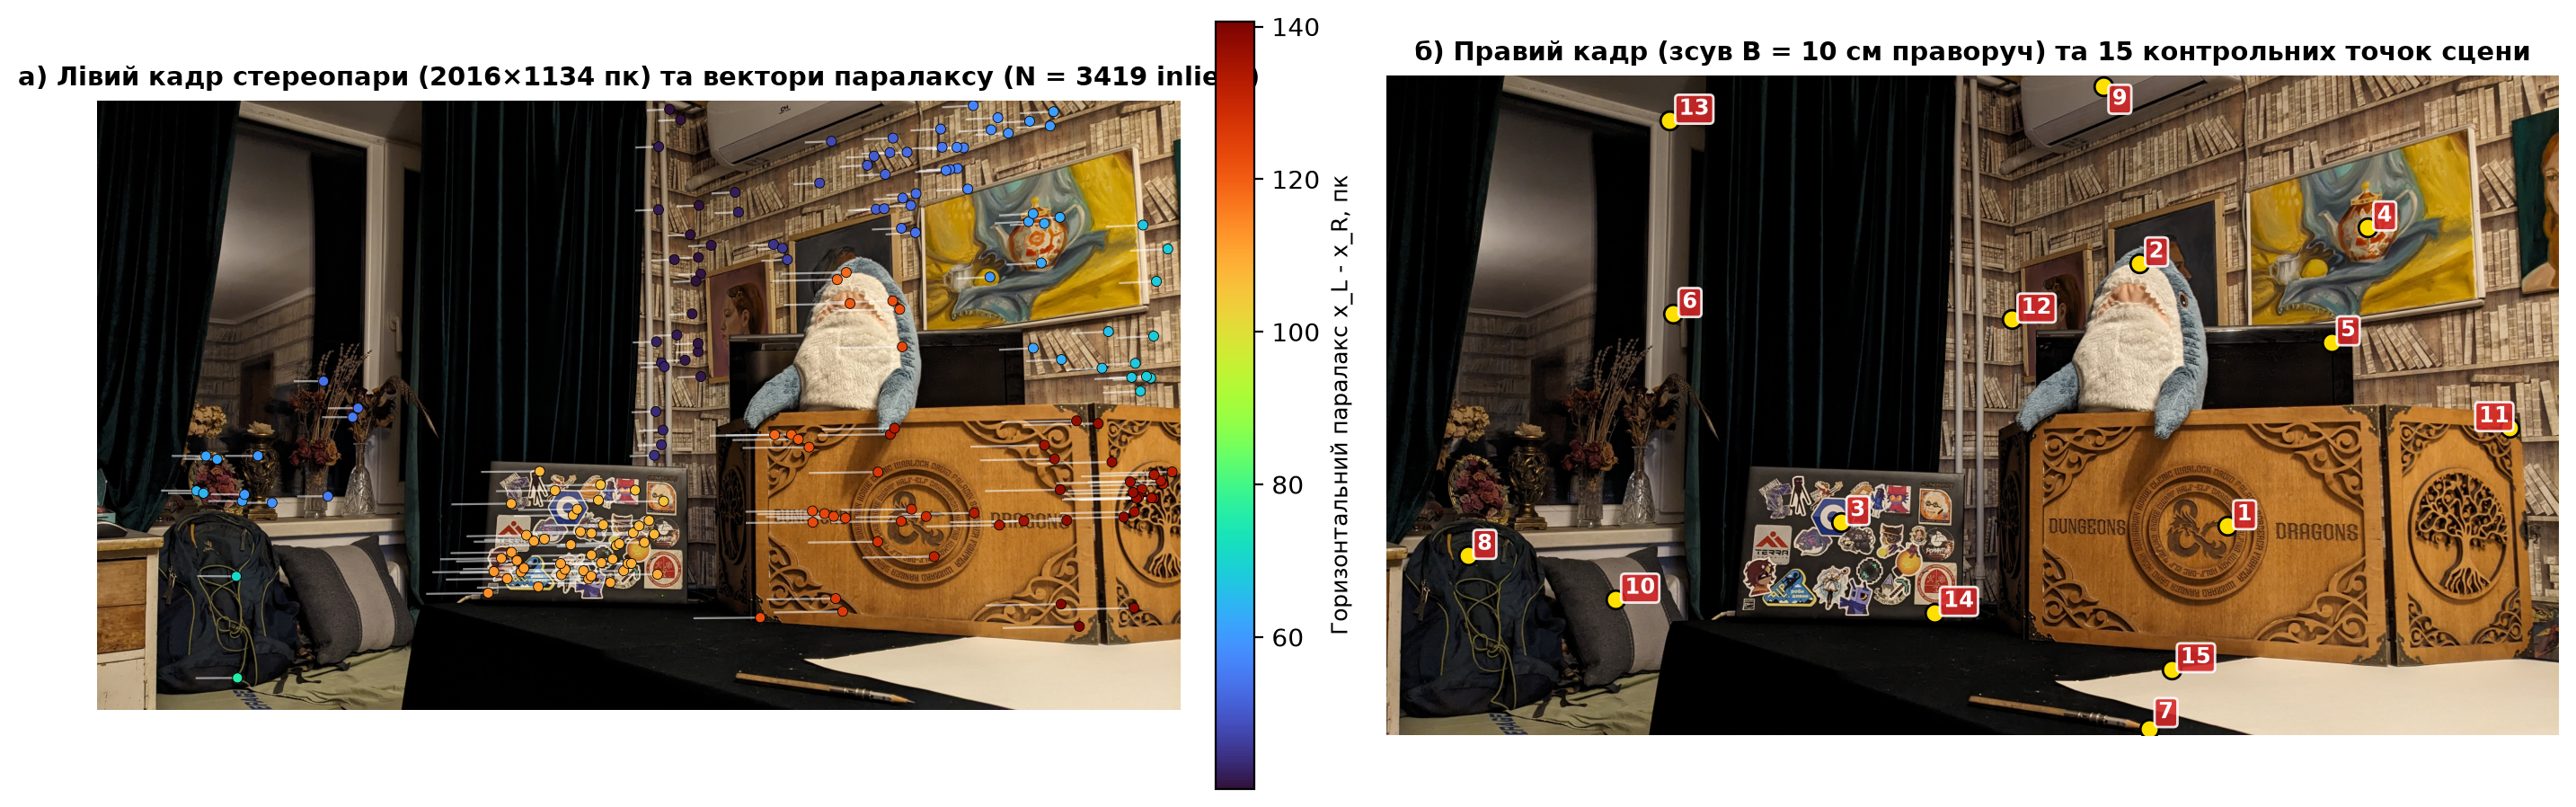
\includegraphics[width=0.98\textwidth]{../figures/a_stereo_input.png}
    \caption{Вхідна стереопара ($2016 \times 1134$~пк, $B = 10$~см): (а) поле векторів горизонтального паралаксу на лівому кадрі ($3419$ inliers); (б) правий кадр із 15 контрольними точками сцени (\texttt{points.svg})}
    \label{fig:stereo_input}
\end{figure}

\begin{table}[htbp]
\centering
\caption{Порівняння моделей взаємного орієнтування стереопари при $B = 100$~мм (Частини A--B, Кроки 3--4)}
\label{tab:stereo_models}
\scriptsize
\setlength{\tabcolsep}{3.5pt}
\begin{tabularx}{\textwidth}{Y r c r r r r}
\toprule
Модель стереопари & $\|\mathbf{r}\|$ & $\mathbf{T} = (T_x; T_y; T_z)$, мм & $f_{\text{rect}}$ & Сер. $|y_L-y_R|$ & Мед. $|y_L-y_R|$ & Частка $<1$~пк \\
\midrule
\directlua{tab_stereo_models()}
\bottomrule
\end{tabularx}
\end{table}

\begin{figure}[htbp]
    \centering
    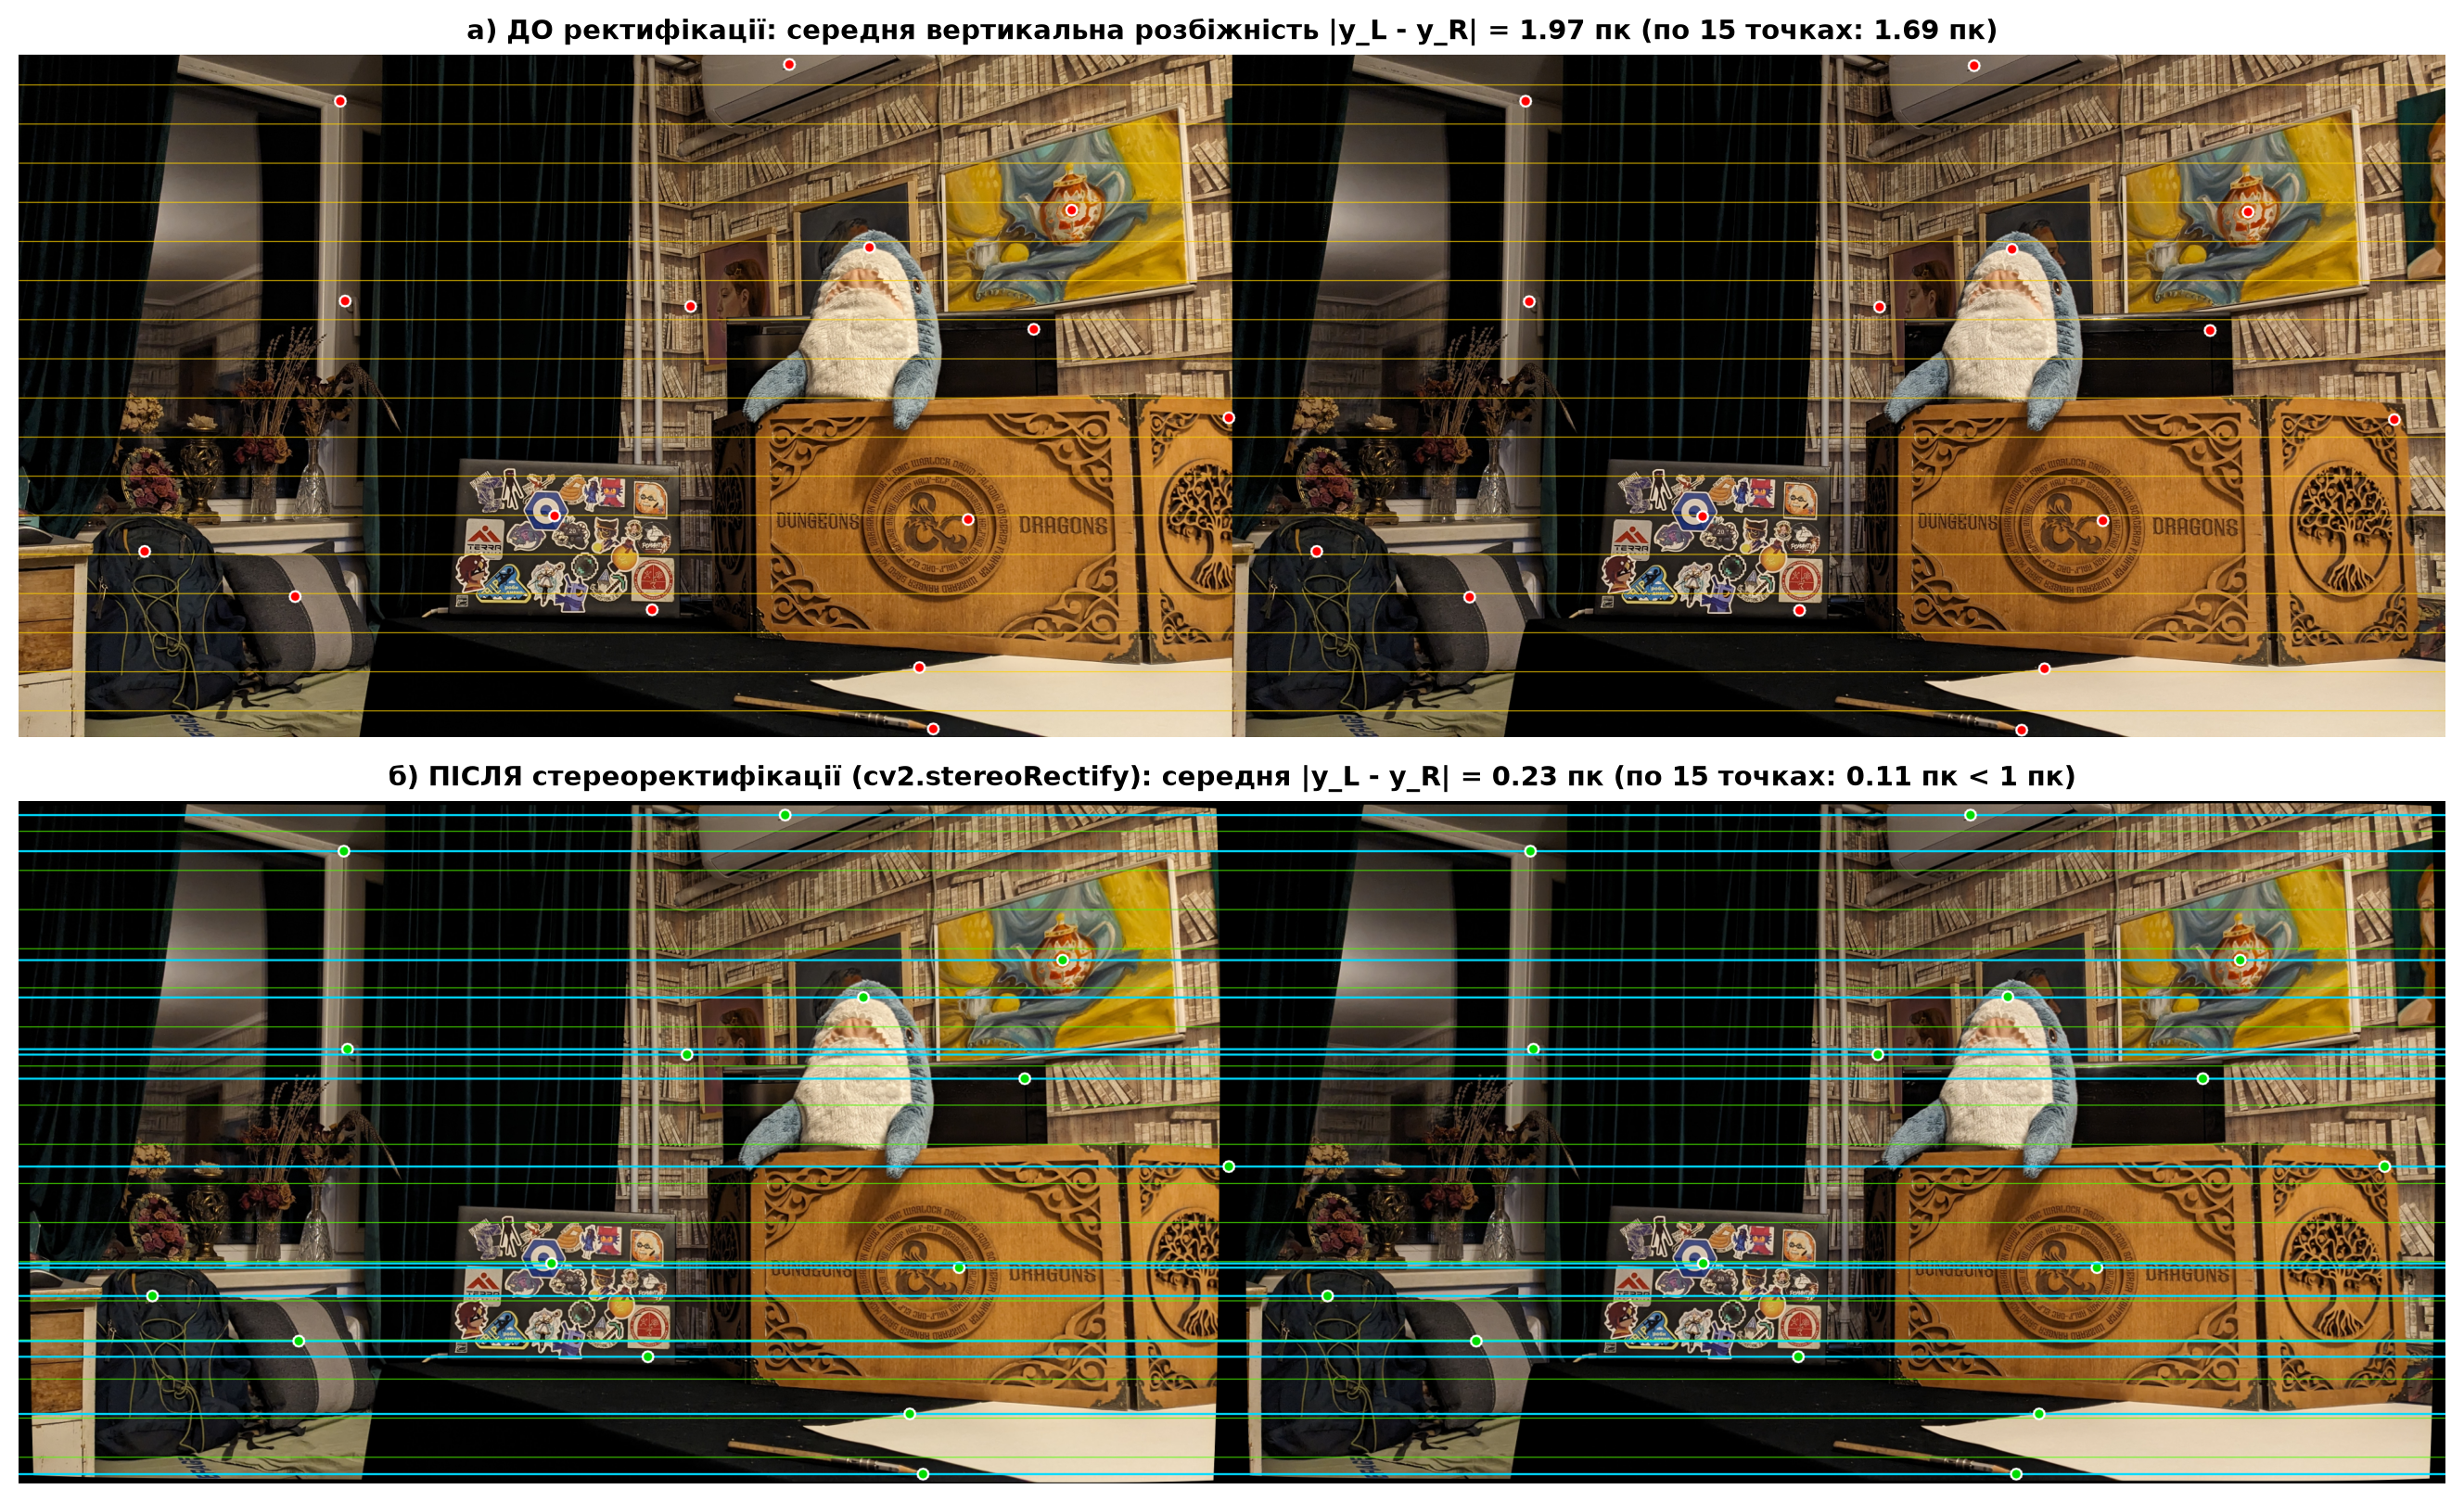
\includegraphics[width=0.96\textwidth]{../figures/b_epipolar_lines.png}
    \caption{Візуальна перевірка епіполярної ректифікації (Крок 5): (а) вхідна стереопара до ректифікації; (б) ректифікована стереопара з вирівнюванням відповідних точок уздовж горизонтальних епіполярних ліній}
    \label{fig:epipolar_lines}
\end{figure}

\begin{table}[htbp]
\centering
\caption{Кількісна перевірка вертикальної розбіжності $|y_L - y_R|$ на 15 контрольних точках (Частина B, Крок 6)}
\label{tab:vertical_discrepancy}
\scriptsize
\setlength{\tabcolsep}{3.5pt}
\begin{tabularx}{\textwidth}{c Y r r r r r r r}
\toprule
\multirow{2}{*}{№} & \multirow{2}{*}{Контрольний об'єкт сцени} & \multicolumn{3}{c}{ДО ректифікації} & \multicolumn{4}{c}{ПІСЛЯ ректифікації} \\
\cmidrule(lr){3-5} \cmidrule(lr){6-9}
 & & $y_L$, пк & $y_R$, пк & $|y_L-y_R|$ & $y_L'$, пк & $y_R'$, пк & $|y_L'-y_R'|$ & $d = x_L'-x_R'$ \\
\midrule
\directlua{tab_vertical_discrepancy()}
\bottomrule
\end{tabularx}
\end{table}

\begin{figure}[htbp]
    \centering
    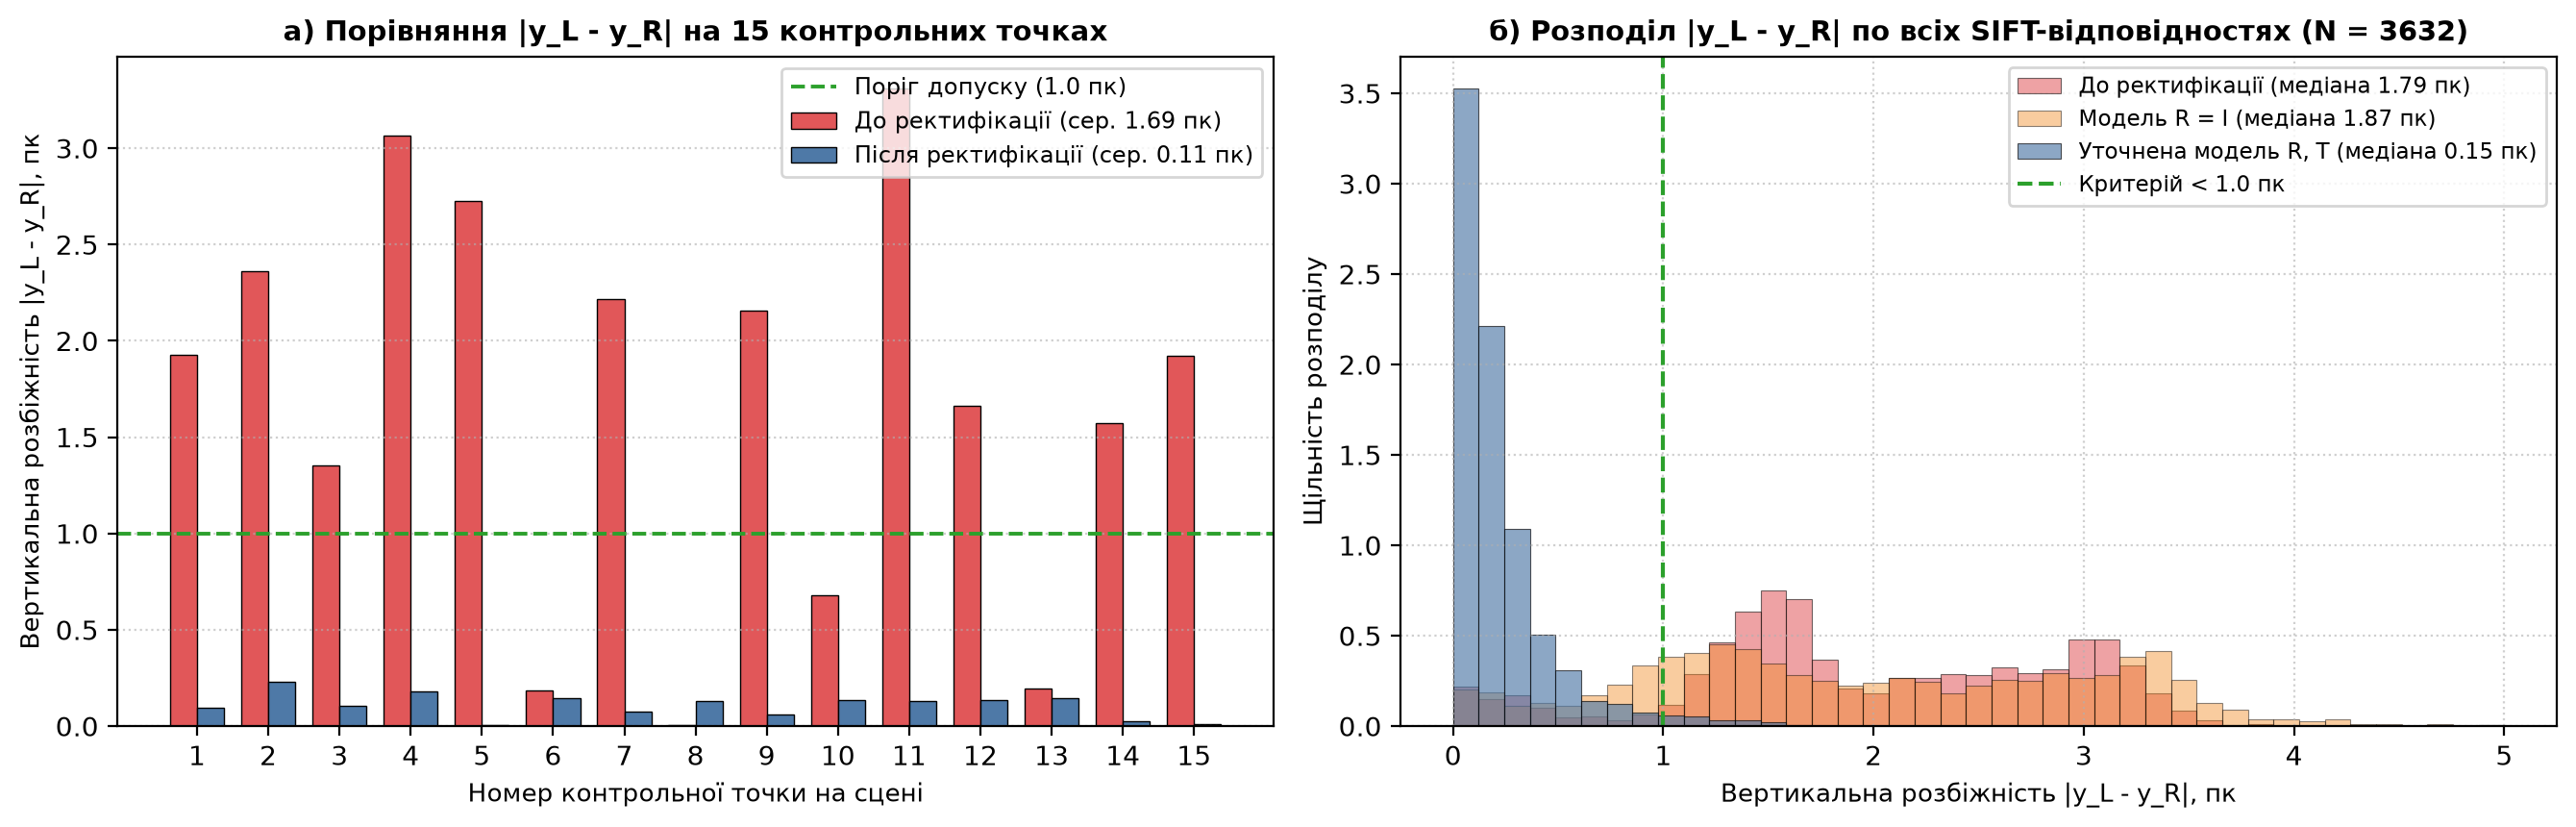
\includegraphics[width=0.98\textwidth]{../figures/b_vertical_discrepancy.png}
    \caption{Кількісна оцінка якості ректифікації (Крок 6): (а) вертикальна розбіжність на 15 контрольних точках сцени; (б) емпіричний розподіл $|y_L - y_R|$ на всій множині SIFT-відповідностей ($N = 3632$)}
    \label{fig:vertical_discrepancy}
\end{figure}

\begin{table}[htbp]
\centering
\caption{Порівняння методів обчислення карти диспаратності (Частина C, Крок 7)}
\label{tab:bm_vs_sgbm}
\scriptsize
\setlength{\tabcolsep}{3.5pt}
\begin{tabularx}{\textwidth}{l c r r r r Y}
\toprule
Метод & $d_{\max}/\text{bs}/\text{ur}$ & Валідні & Час & Шум $\nabla^2 d$ & MAE SIFT & Характеристика карти \\
\midrule
\directlua{tab_bm_vs_sgbm()}
\bottomrule
\end{tabularx}
\end{table}

\begin{figure}[htbp]
    \centering
    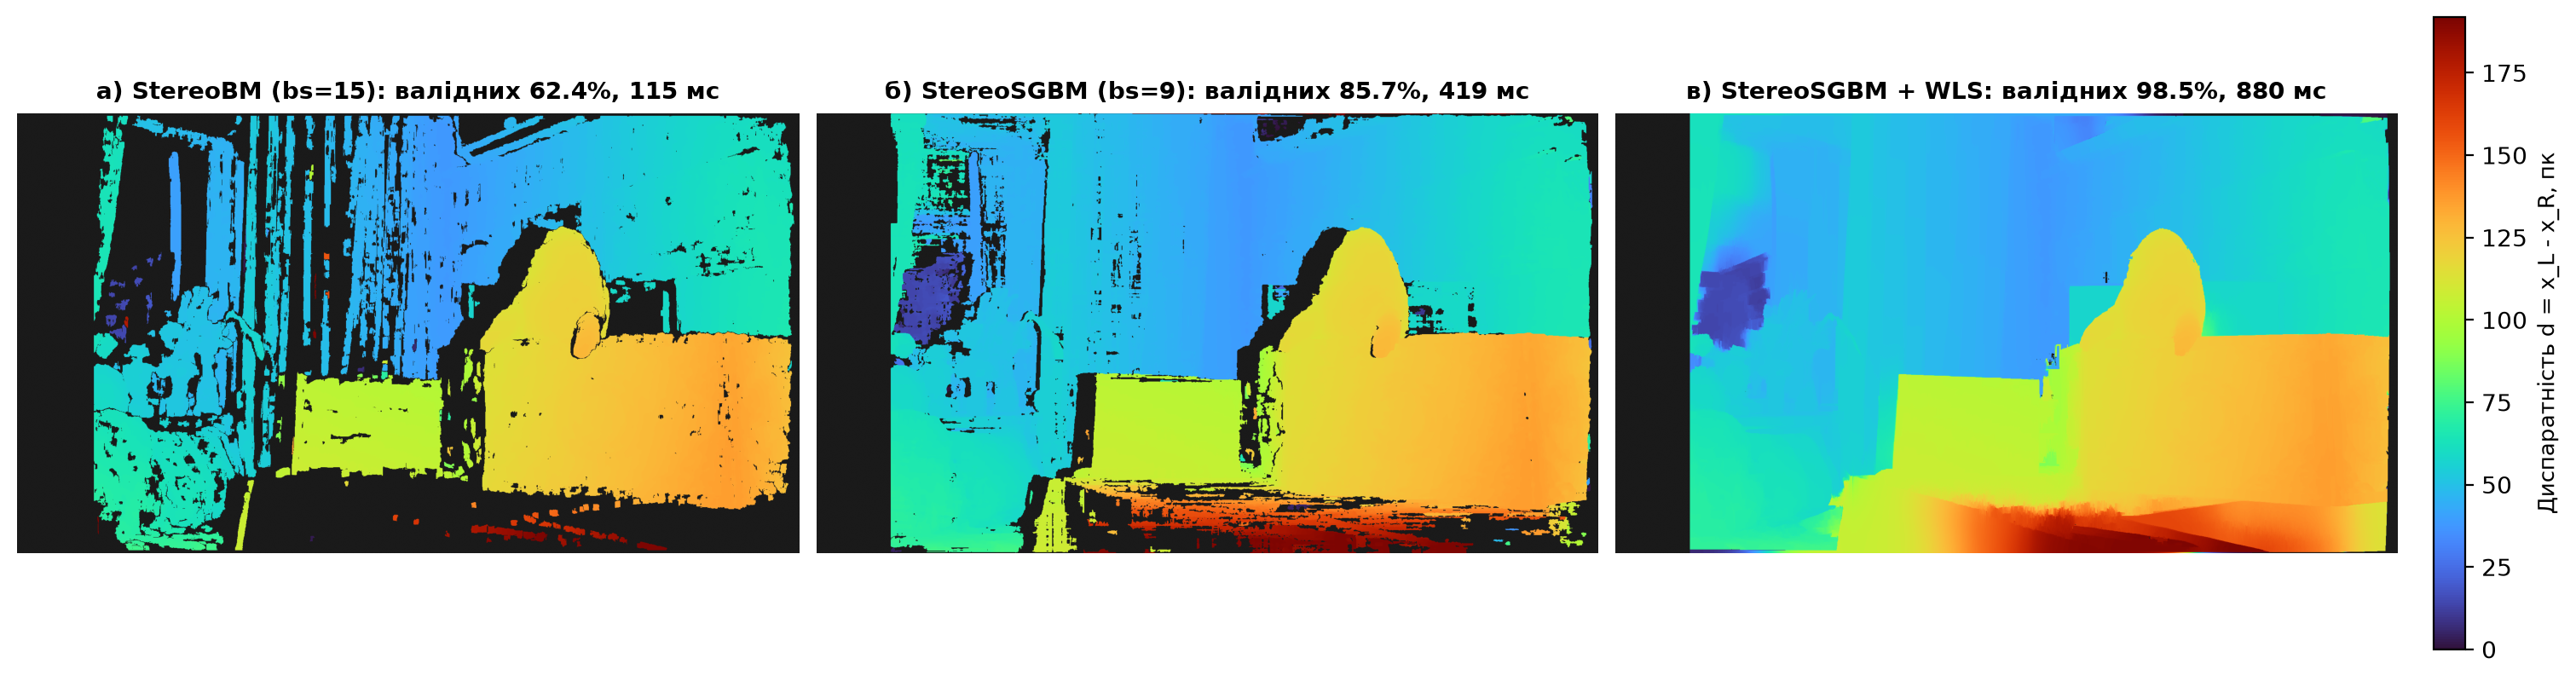
\includegraphics[width=0.98\textwidth]{../figures/c_bm_vs_sgbm.png}
    \caption{Візуальне порівняння карт диспаратності (Крок 7): (а) локальний метод \texttt{StereoBM}; (б) напівглобальний метод \texttt{StereoSGBM}; (в) \texttt{StereoSGBM} із постфільтрацією WLS}
    \label{fig:bm_vs_sgbm}
\end{figure}

\begin{table}[htbp]
\centering
\caption{Вплив параметрів \texttt{StereoSGBM} на повноту, швидкодію та точність карти диспаратності (Частина C, Крок 8)}
\label{tab:grid_summary}
\scriptsize
\setlength{\tabcolsep}{3.5pt}
\begin{tabularx}{\textwidth}{c c c r r r r Y}
\toprule
\texttt{numDisp} & \texttt{blockSize} & \texttt{uniqRatio} & Валідні & Час & Шум $\nabla^2 d$ & MAE SIFT & Візуальна оцінка якості \\
\midrule
\directlua{tab_grid_summary()}
\bottomrule
\end{tabularx}
\end{table}

\begin{figure}[htbp]
    \centering
    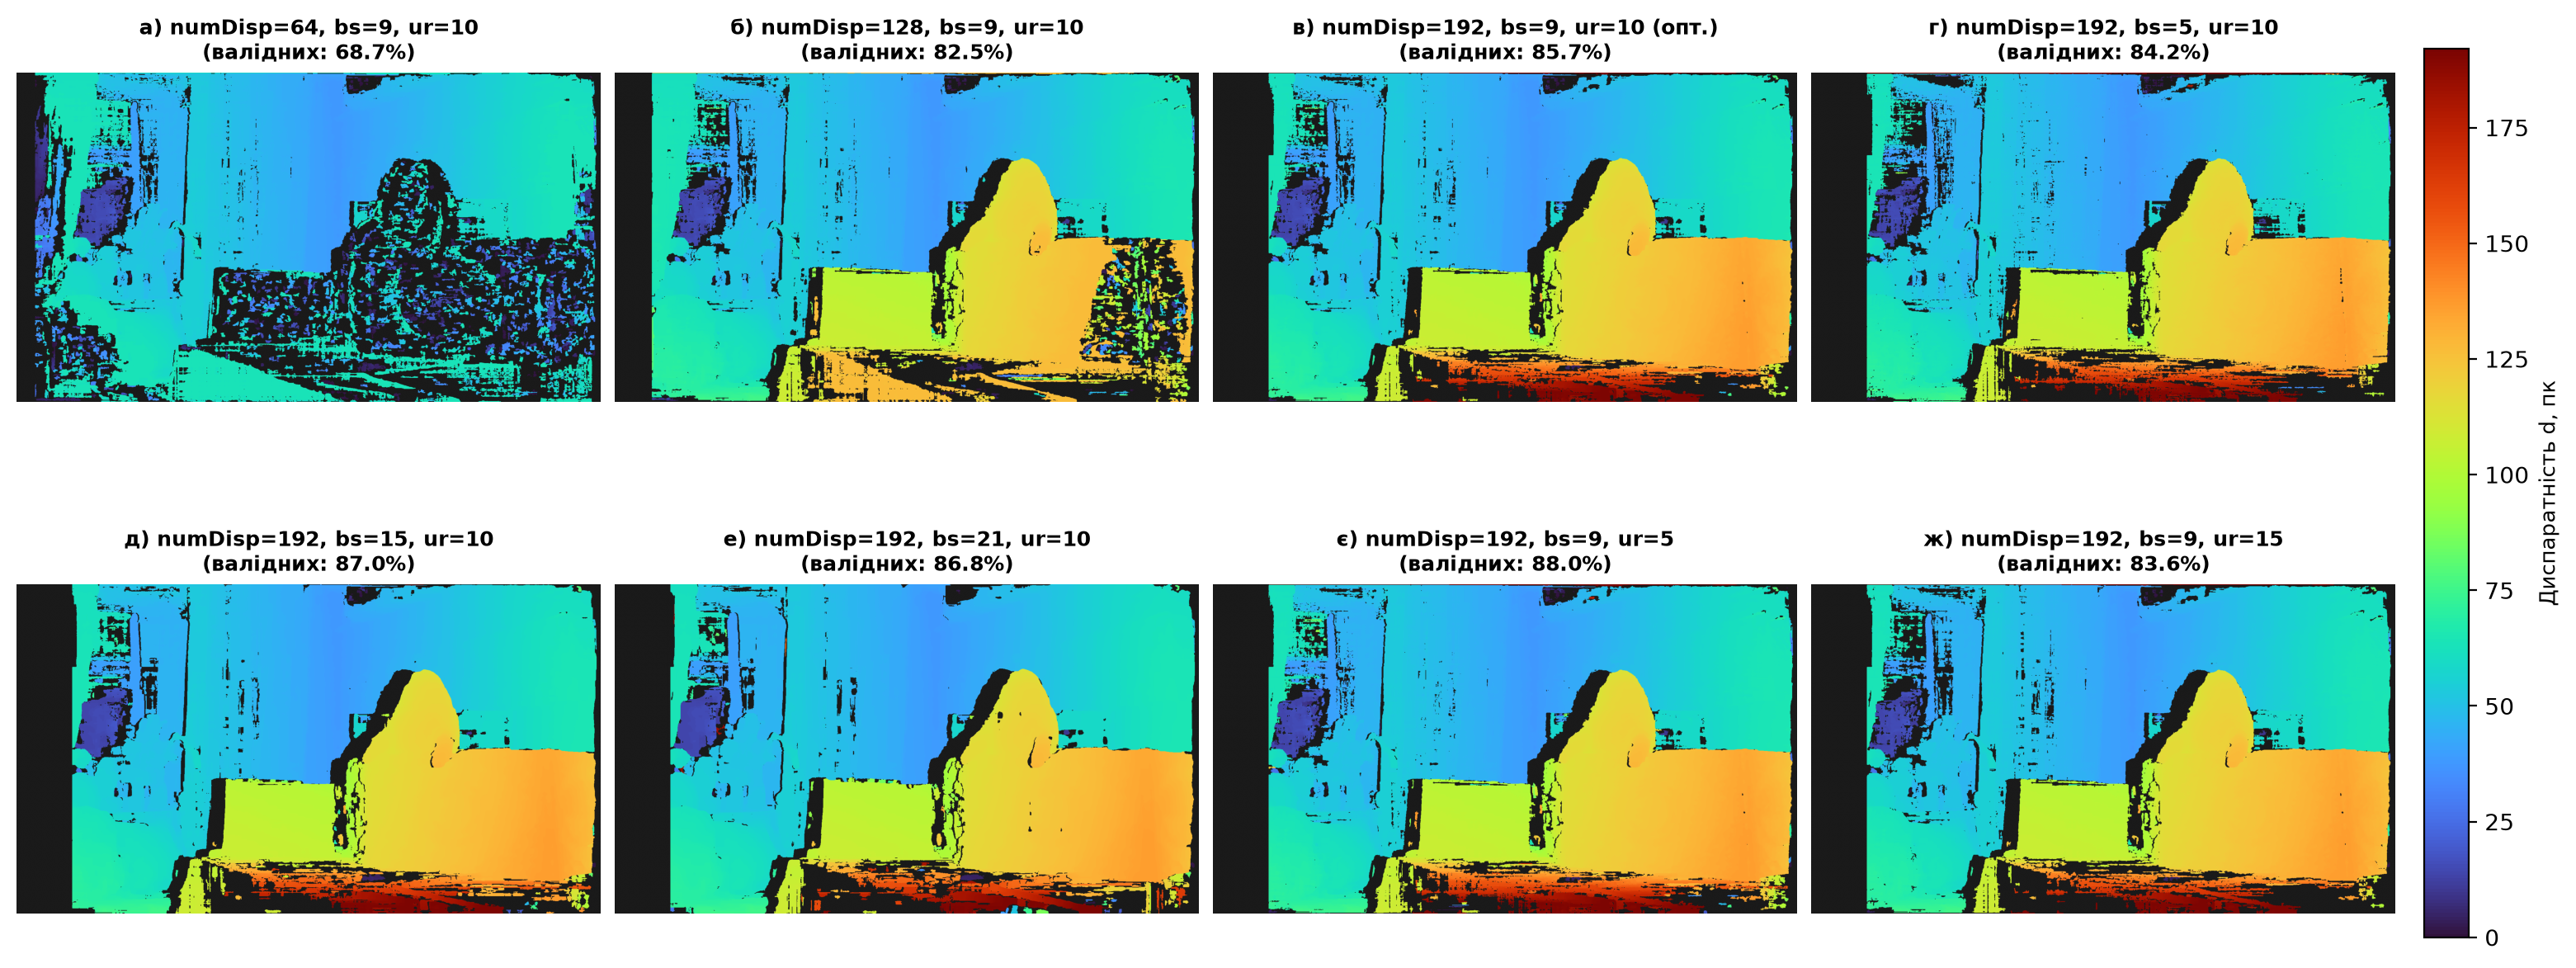
\includegraphics[width=0.98\textwidth]{../figures/c_grid_maps.png}
    \caption{Порівняння карт диспаратності \texttt{StereoSGBM} при варіації параметрів \texttt{numDisparities}, \texttt{blockSize} та \texttt{uniquenessRatio} (Крок 8)}
    \label{fig:grid_maps}
\end{figure}

\begin{figure}[htbp]
    \centering
    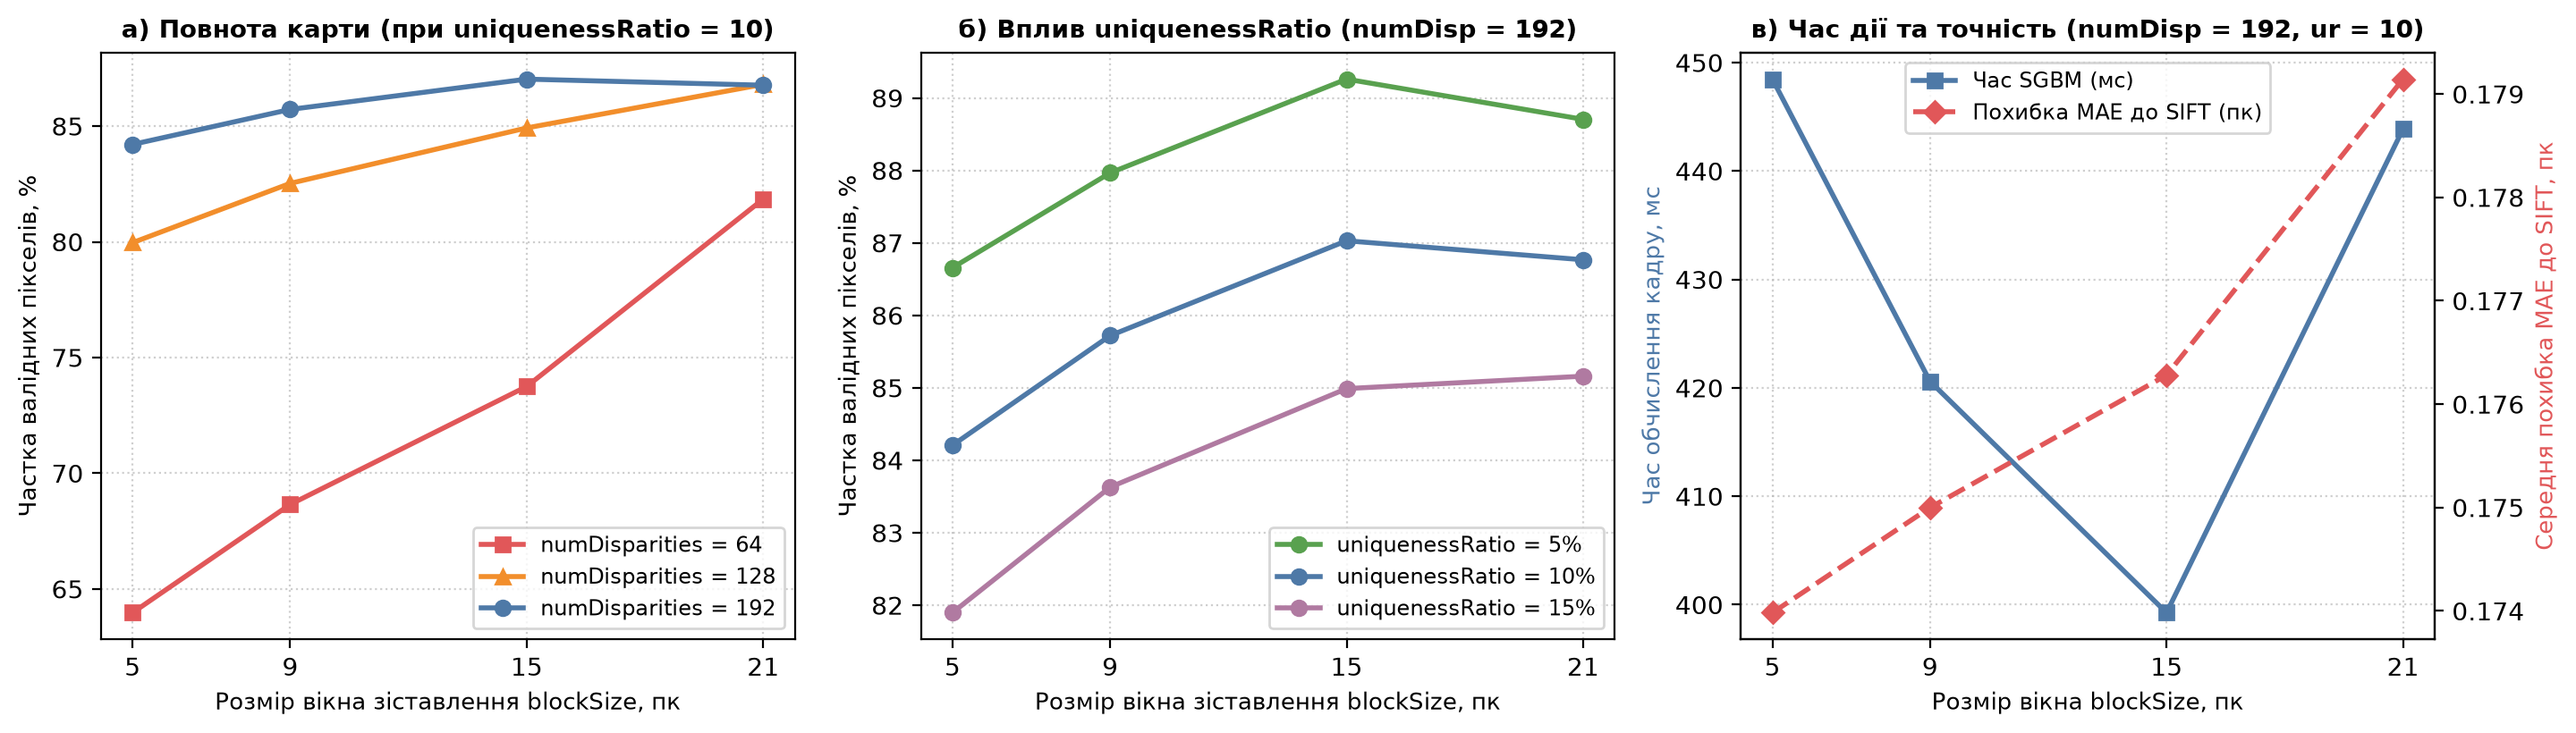
\includegraphics[width=0.98\textwidth]{../figures/c_grid_analysis.png}
    \caption{Кількісні залежності характеристик карти диспаратності від параметрів \texttt{StereoSGBM} (Крок 8): (а) вплив \texttt{numDisparities} та \texttt{blockSize}; (б) вплив \texttt{uniquenessRatio}; (в) час обчислення та похибка MAE}
    \label{fig:grid_analysis}
\end{figure}

\begin{figure}[htbp]
    \centering
    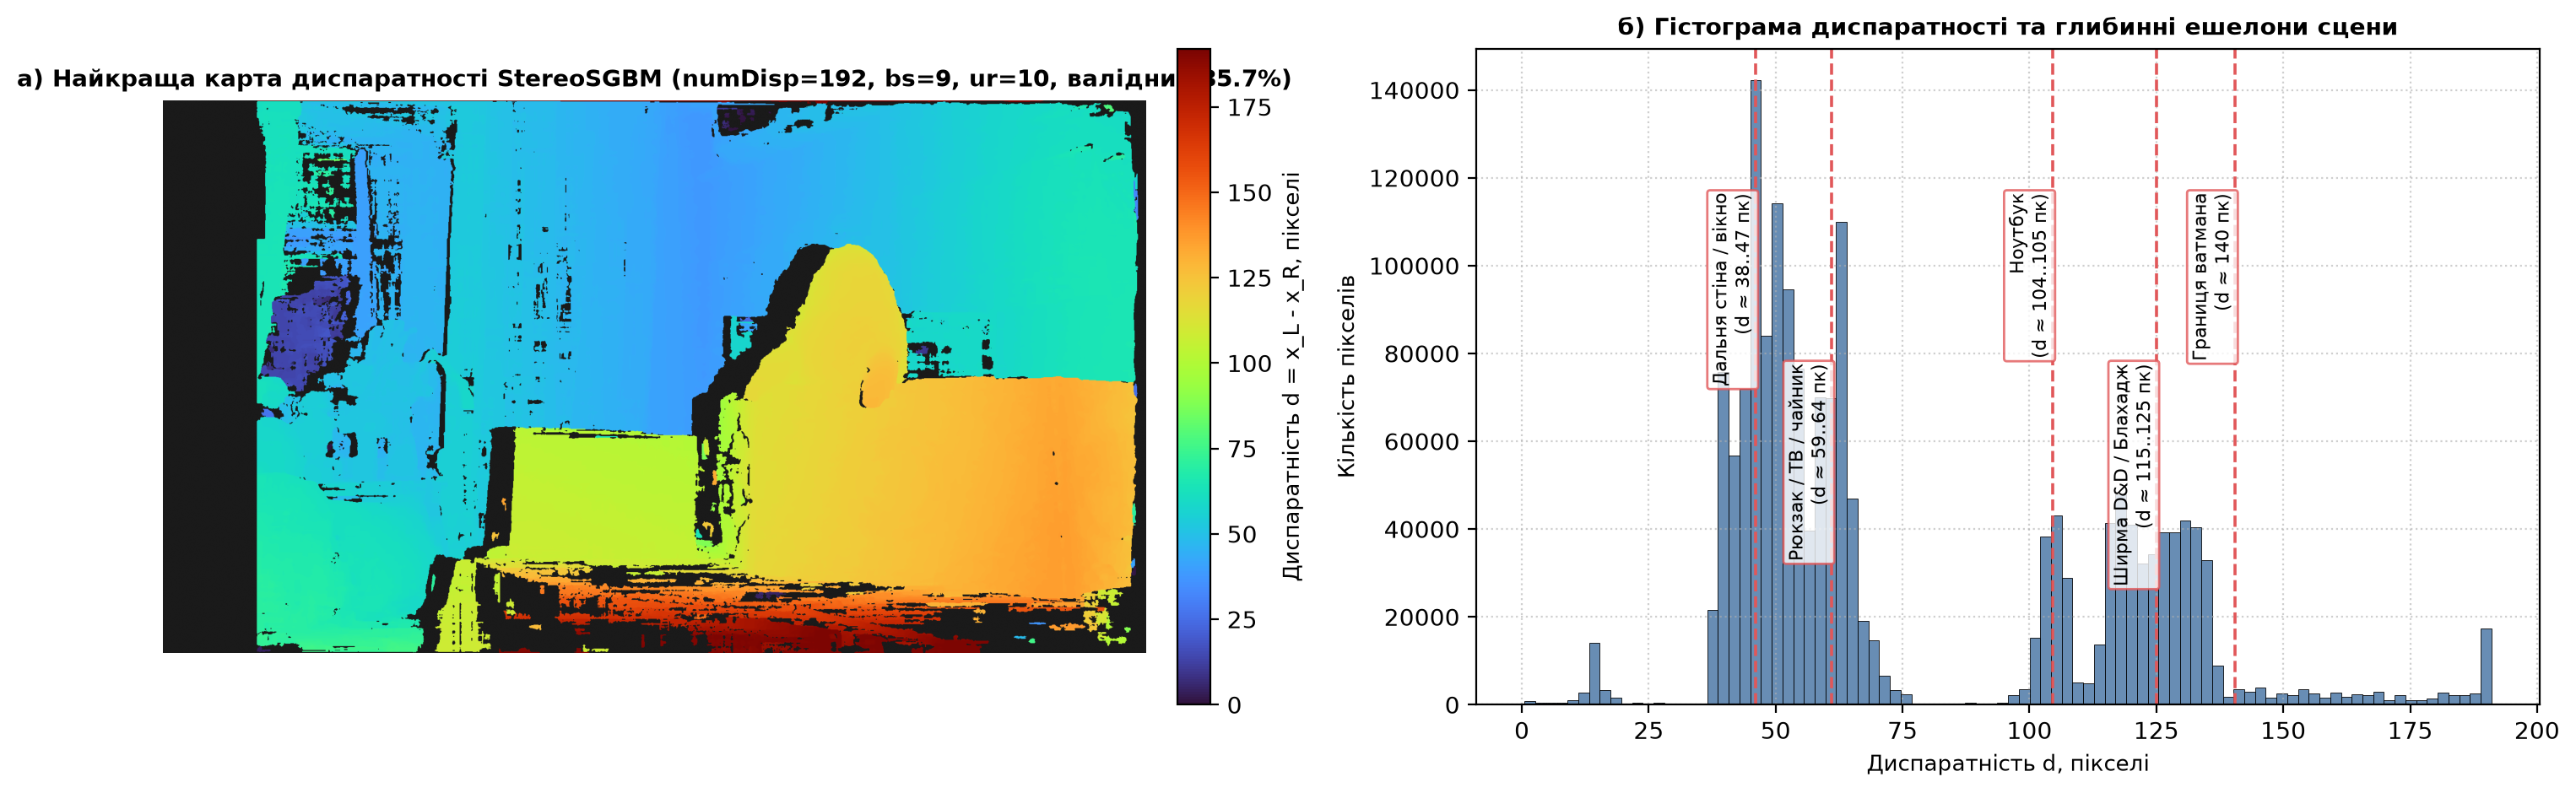
\includegraphics[width=0.98\textwidth]{../figures/c_best_disparity.png}
    \caption{Найкраща карта диспаратності \texttt{StereoSGBM} ($\texttt{numDisparities} = 192, \texttt{blockSize} = 9, \texttt{uniquenessRatio} = 10$) із каліброваною шкалою у пікселях (а) та гістограма розподілу диспаратності за ешелонами сцени (б) (Крок 9)}
    \label{fig:best_disparity}
\end{figure}

\begin{table}[htbp]
\centering
\caption{Верифікація обчисленої стереоглибини $Z_{\text{calc}}$ за 15 контрольними точками сцени (Частина D, Крок 11)}
\label{tab:depth_verification}
\scriptsize
\setlength{\tabcolsep}{3.5pt}
\begin{tabularx}{\textwidth}{c Y c r r r r r}
\toprule
№ & Контрольна точка сцени & Коорд. $(x; y)$ & $d \pm \sigma_d$, пк & $Z_{\text{meas}}$ & $Z_{\text{calc}}$ & $|\Delta Z|$ & $\delta_Z$ \\
\midrule
\directlua{tab_depth_verification()}
\bottomrule
\end{tabularx}
\end{table}

\begin{figure}[htbp]
    \centering
    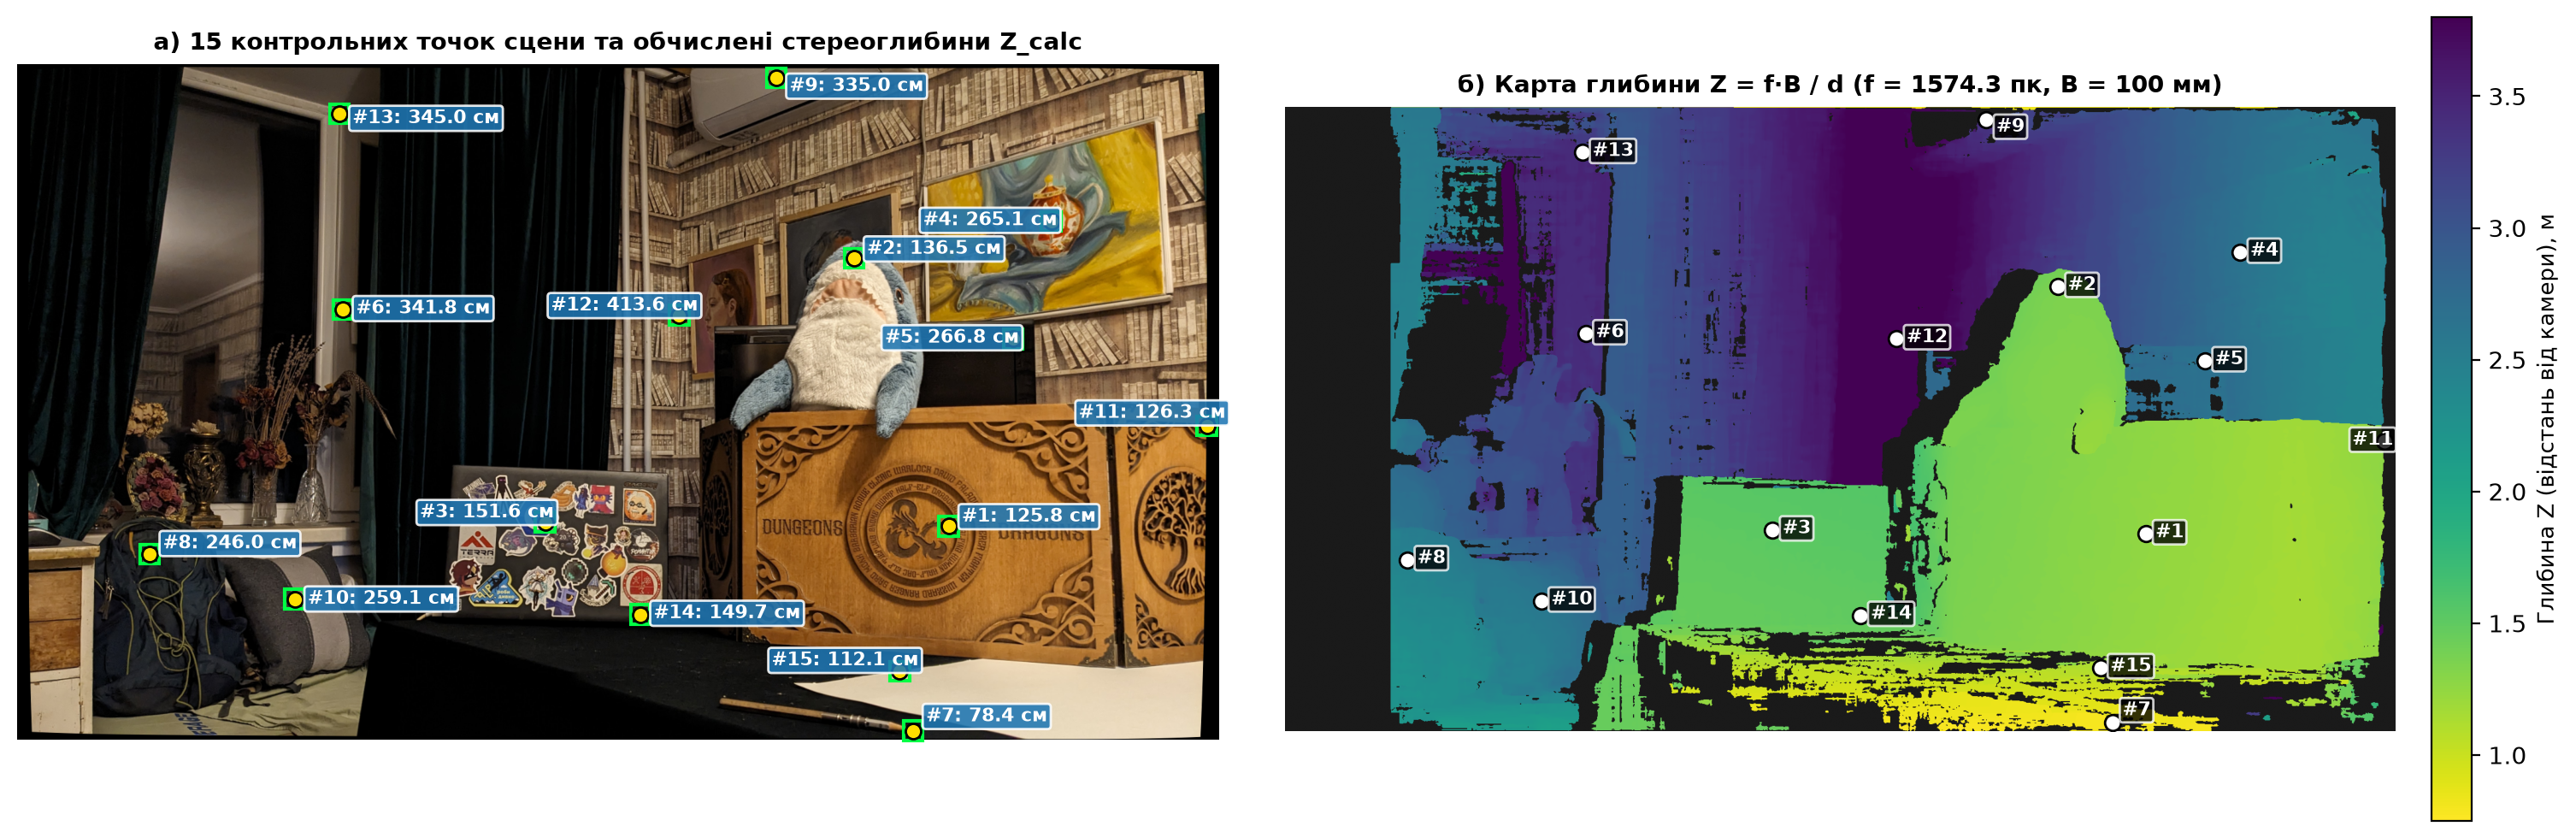
\includegraphics[width=0.98\textwidth]{../figures/d_depth_map.png}
    \caption{Метрична реконструкція глибини (Крок 11): (а) розташування 15 контрольних точок у кадрі; (б) карта глибини $Z$ у метрах із кольоровою шкалою}
    \label{fig:depth_map}
\end{figure}

\begin{figure}[htbp]
    \centering
    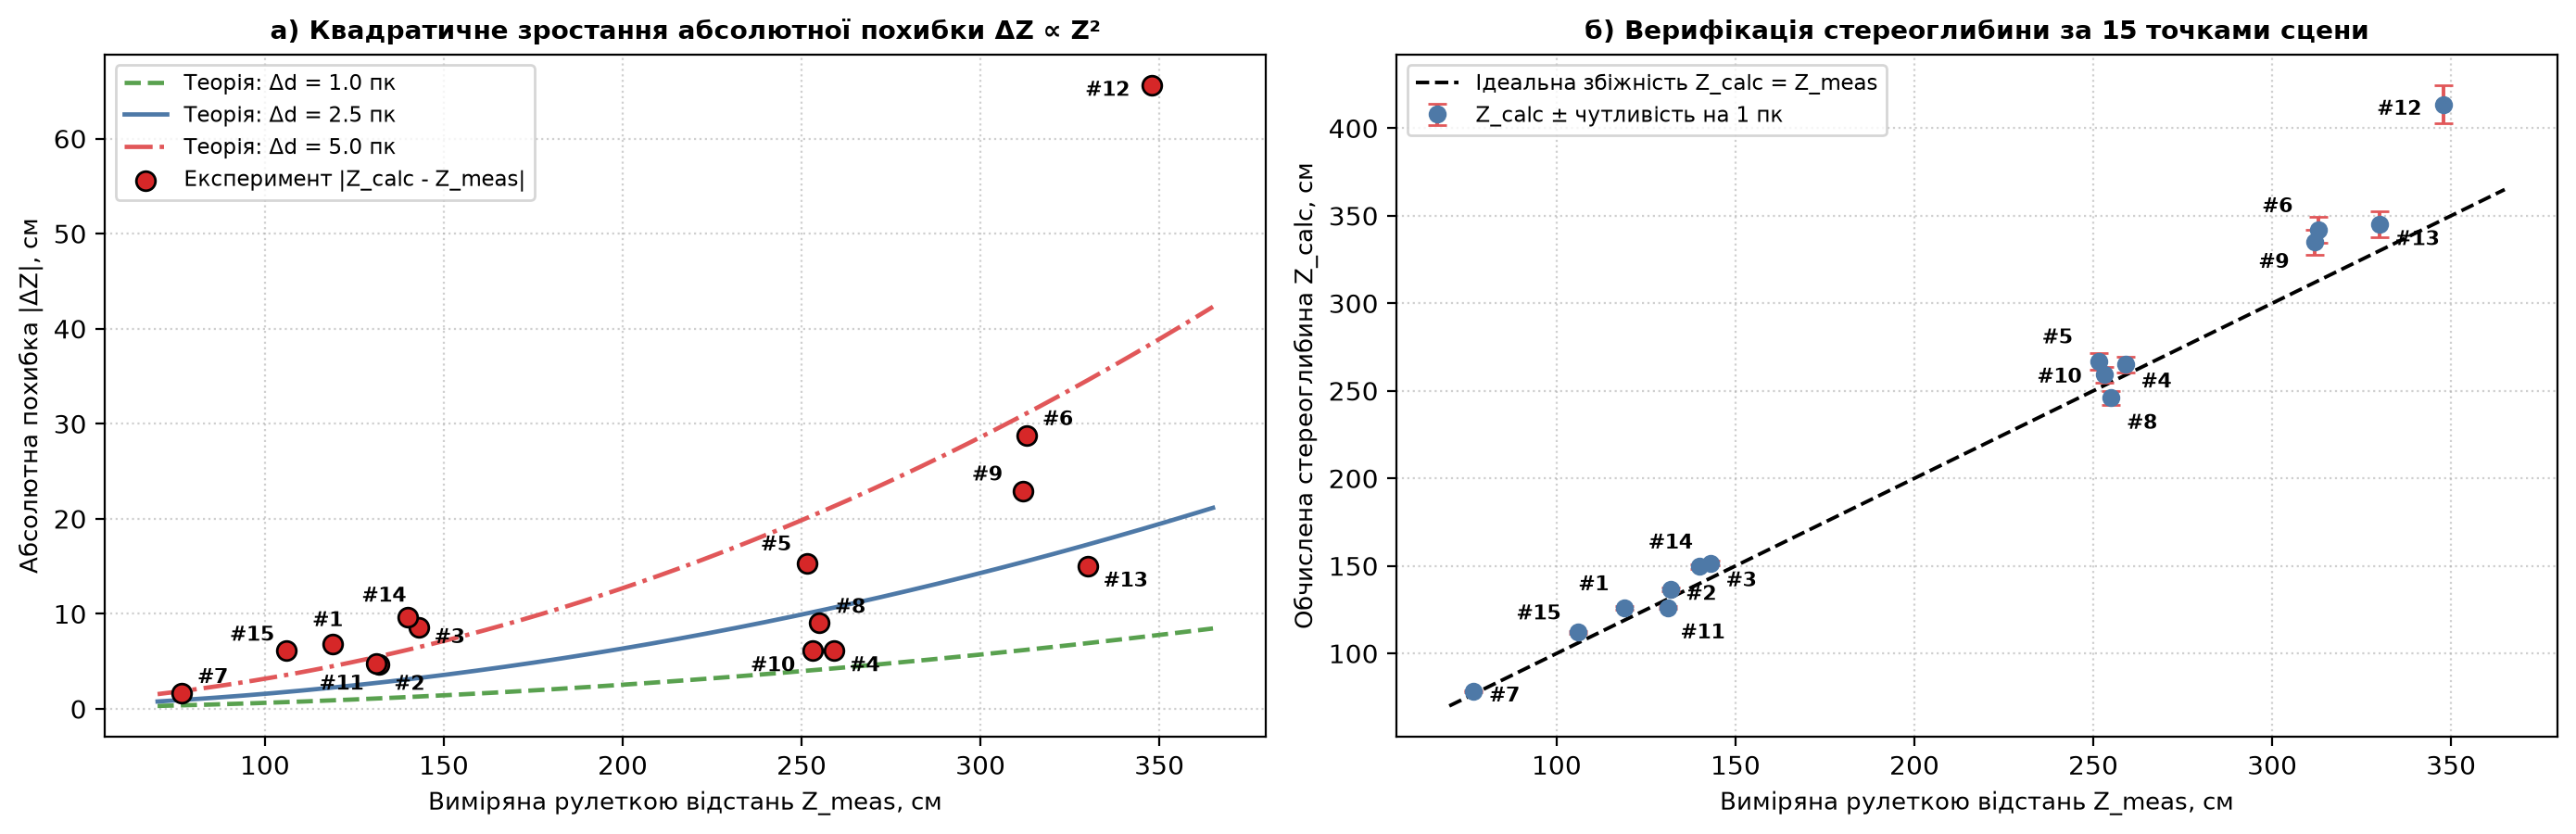
\includegraphics[width=0.98\textwidth]{../figures/d_error_vs_distance.png}
    \caption{Аналіз точності вимірювання відстані (Крок 11): (а) зіставлення експериментальної похибки $|\Delta Z|$ з теоретичними кривими $\Delta Z(Z) = \frac{Z^2}{fB}\Delta d$; (б) лінійність залежності $Z_{\text{calc}}(Z_{\text{meas}})$ на 15 точках сцени}
    \label{fig:error_vs_distance}
\end{figure}

\begin{figure}[htbp]
    \centering
    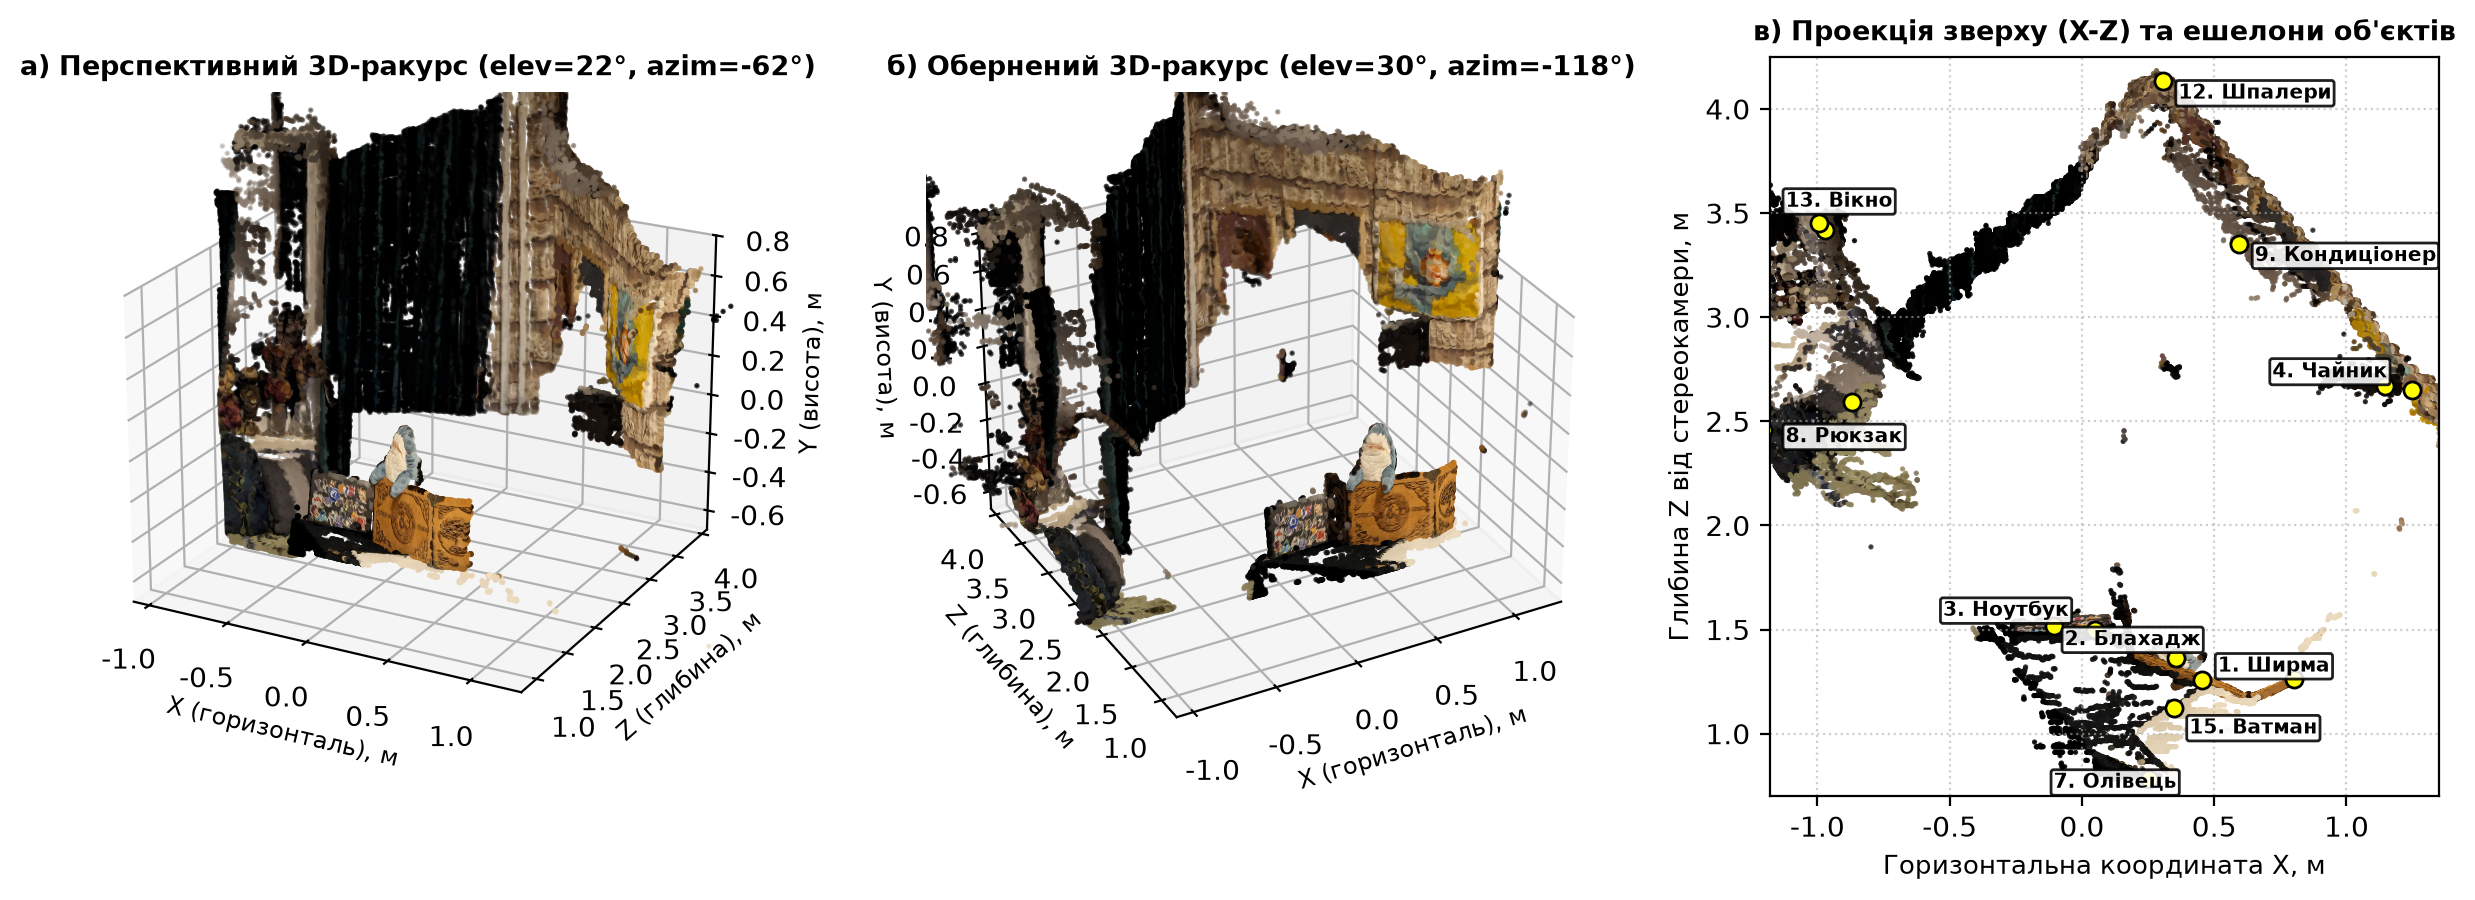
\includegraphics[width=0.98\textwidth]{../figures/d_point_cloud.png}
    \caption{Реконструйована 3D-хмара точок сцени (Крок 12, $411\,740$ вершин): (а, б) перспективні тривимірні ракурси; (в) вид зверху у площині $(X, Z)$ з позначеними ешелонами об'єктів}
    \label{fig:point_cloud}
\end{figure}

\begin{table}[htbp]
\centering
\caption{Кількісна характеристика зон систематичних помилок стереозіставлення (Частина E, Крок 14)}
\label{tab:error_zones}
\scriptsize
\setlength{\tabcolsep}{3.0pt}
\begin{tabularx}{\textwidth}{c >{\raggedright\arraybackslash}p{2.2cm} >{\raggedright\arraybackslash}p{2.3cm} r r Y Y}
\toprule
Зона & Тип помилки & Локалізація у сцені & Дірки BM & Дірки SGBM & Фізична / алгоритмічна причина & Спосіб зменшення похибки \\
\midrule
\directlua{tab_error_zones()}
\bottomrule
\end{tabularx}
\end{table}

\begin{figure}[htbp]
    \centering
    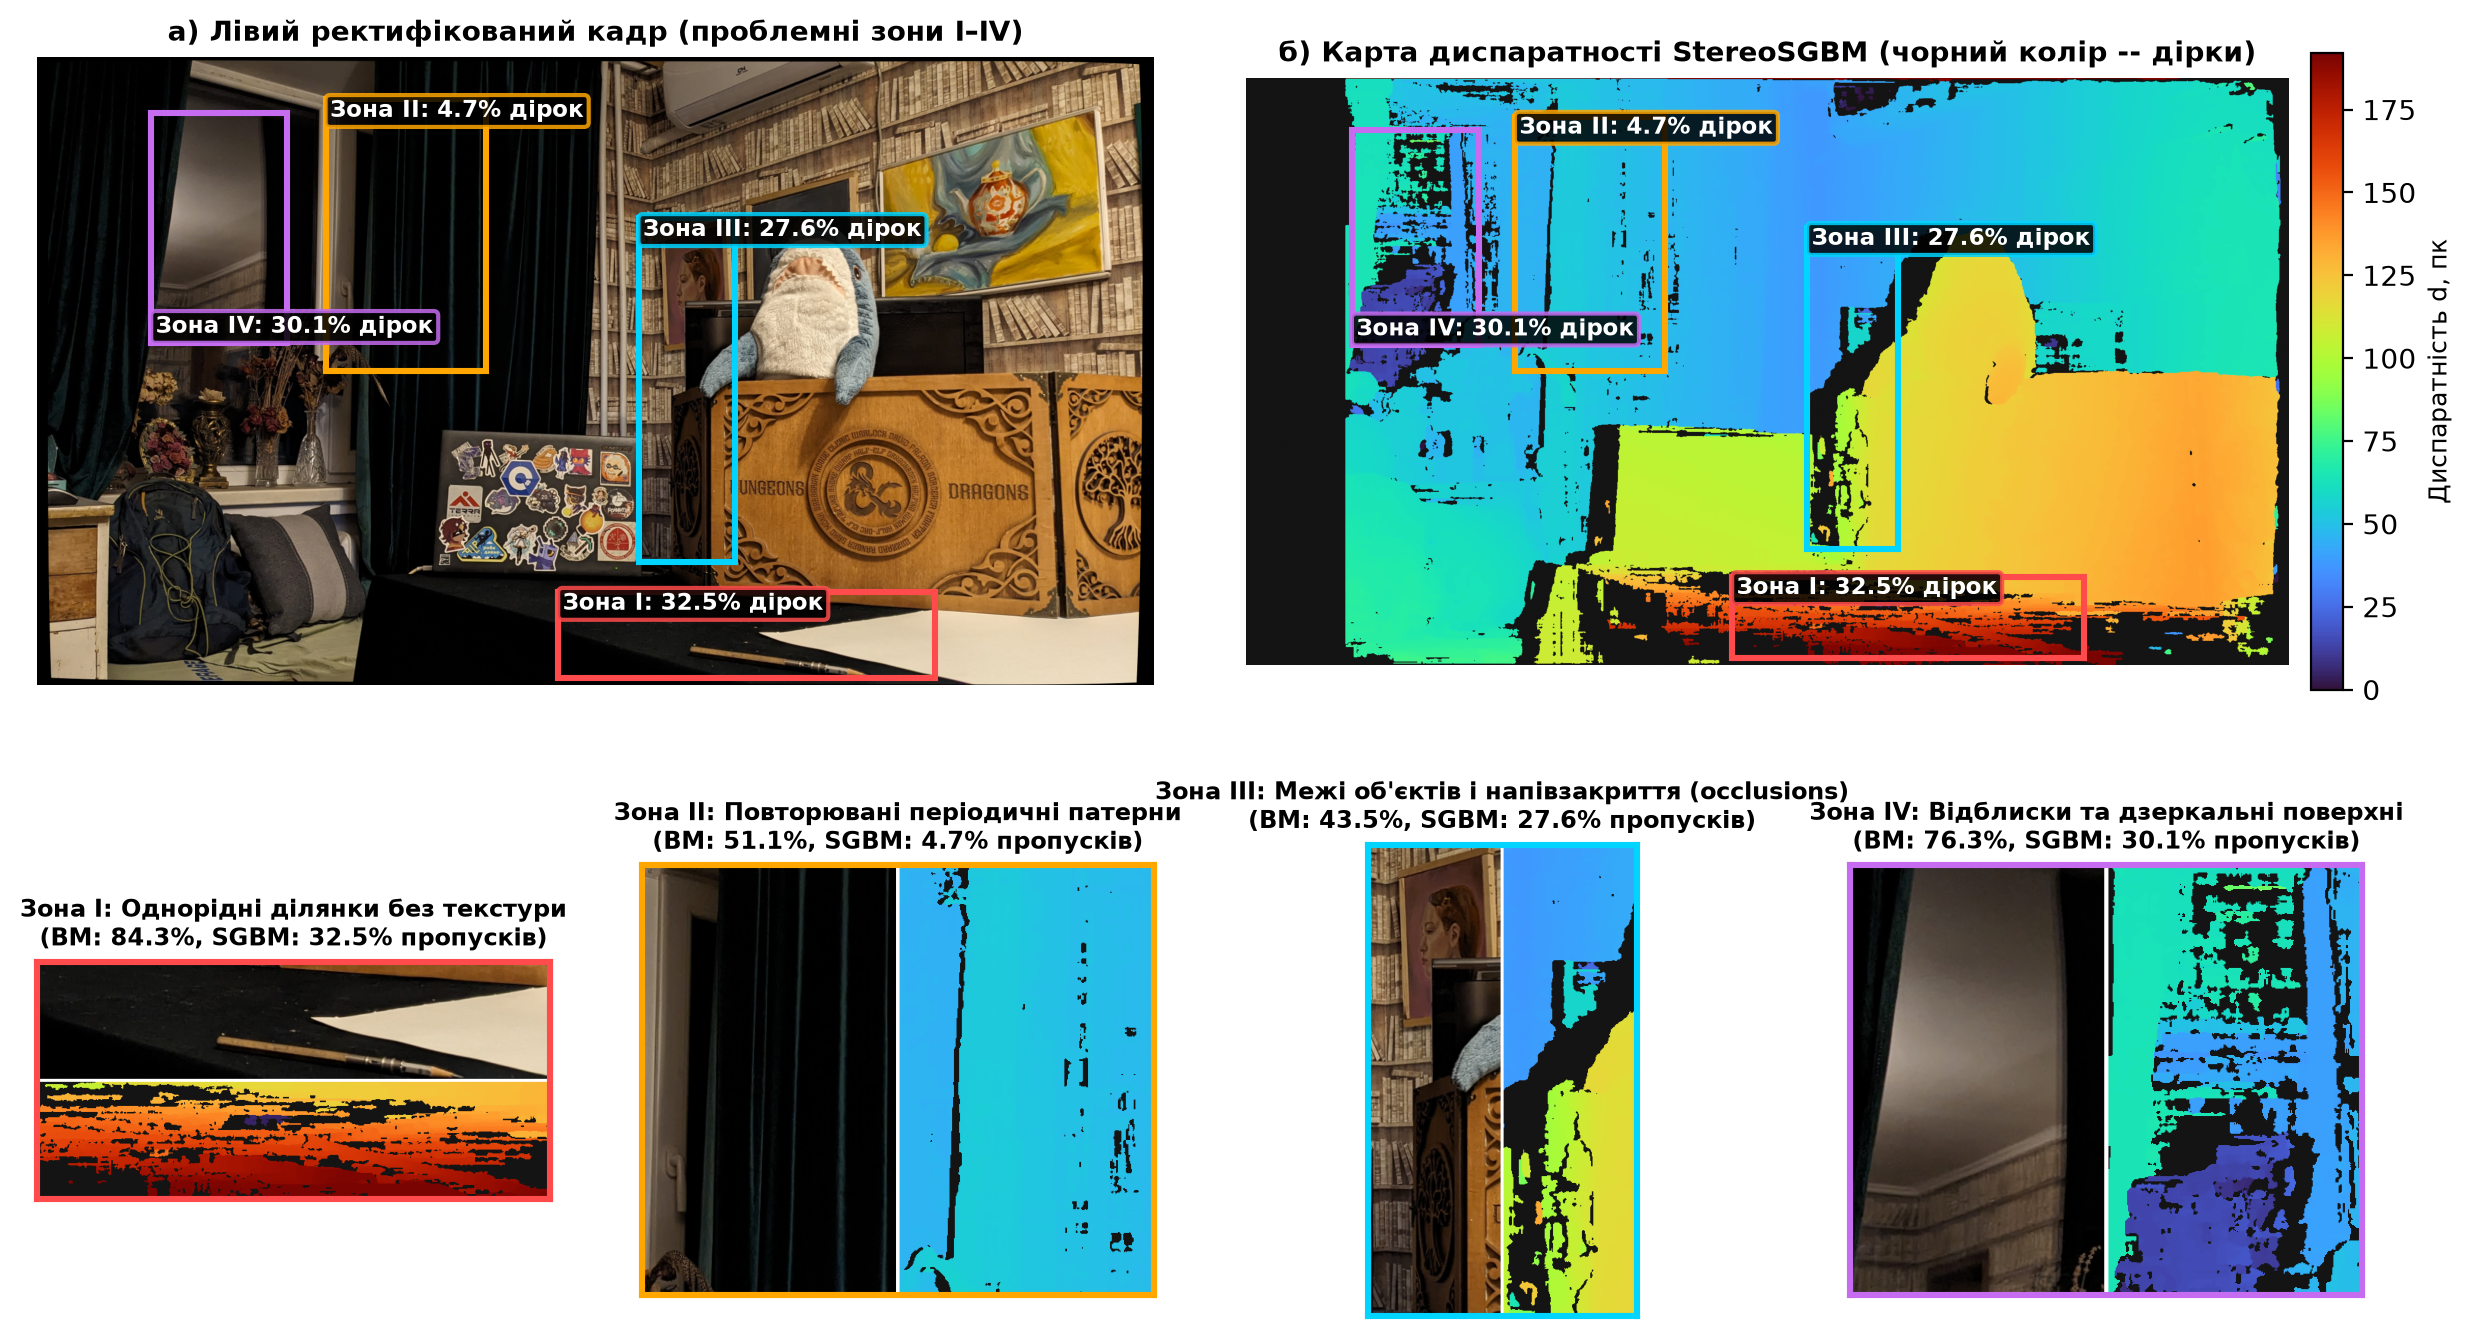
\includegraphics[width=0.98\textwidth]{../figures/e_systematic_errors.png}
    \caption{Систематичні помилки стереозіставлення (Крок 14): (а, б) локалізація чотирьох проблемних зон I--IV на RGB-кадрі та карті диспаратності \texttt{StereoSGBM}; (внизу) збільшені фрагменти зон I--IV}
    \label{fig:systematic_errors}
\end{figure}

\newpage
\section{Аналіз результатів}
\begin{enumerate}
    \item \textbf{Узгодження калібрувальних параметрів та точність епіполярної ректифікації (Частини A, B)}: як свідчать дані Таблиці~\ref{tab:stereo_models}, під час ручного горизонтального переміщення смартфона на базу $B = 100.0$~мм фактичний кут взаємного повороту камер склав лише $\|\mathbf{r}\| = 0.160^\circ$ ($\mathbf{r} = (-0.043^\circ, -0.082^\circ, +0.131^\circ)^T$), а відновлений за істотною матрицею $E$ вектор переносу $\mathbf{T} = (-100.00, +0.07, -0.30)^T$~мм на $99.999\%$ відповідає чисто горизонтальному зсуву вздовж осі $O X$. Проте при фокусній відстані $f_{\text{rect}} = 1574.27$~пк навіть мікроскопічний тангаж і крен у $0.08^\circ$--$0.13^\circ$ створюють вертикальний зсув проєкцій $\Delta y \approx f \sin(0.08^\circ) \approx 2.2$~пк, тому номінальна ректифікація з ідеалізованою матрицею $R = I_3$ залишає середню вертикальну похибку $1.977$~пк (частка точок із $|y_L - y_R| < 1$~пк становить лише $19.2\%$). Компенсація мікроповороту $R$ у \texttt{cv2.stereoRectify} ($\alpha = -1$) знижує середню вертикальну розбіжність по всіх $3632$ точках SIFT майже у дев'ять разів -- до $\mathbf{0.225}$~пк (медіана -- $\mathbf{0.147}$~пк, частка точок із похибкою $< 1$~пк досягає $\mathbf{97.5\%}$), а на 15 контрольних точках різних ешелонів сцени середня похибка зменшується з $1.69$~пк до $\mathbf{0.11}$~пк при максимумі $0.23$~пк (Таблиця~\ref{tab:vertical_discrepancy}, Рис.~\ref{fig:vertical_discrepancy}).

    \item \textbf{Порівняння алгоритмів \texttt{StereoBM} та \texttt{StereoSGBM} (Частина C, Крок 7)}: локальний алгоритм блокового зіставлення \texttt{StereoBM} ($\text{blockSize} = 15$) працює у $3.6$ раза швидше за напівглобальний метод ($115.5$~мс проти $419.5$~мс, Таблиця~\ref{tab:bm_vs_sgbm}), але забезпечує лише $62.4\%$ валідних пікселів, утворюючи великі лакуни на однорідній поверхні столу, білому аркуші ватмана, темній шторі та склі вікна (Рис.~\ref{fig:bm_vs_sgbm}а). Напівглобальна оптимізація \texttt{StereoSGBM} ($\text{blockSize} = 9$) за рахунок поширення штрафів гладкості $P_1, P_2$ з інформативних контурів на сусідні слаботекстуровані ділянки підвищує повноту карти до $\mathbf{85.7\%}$, зменшує високочастотну градієнтну шорсткість площин з $0.080$~пк до $\mathbf{0.064}$~пк і забезпечує субпіксельну точність $\text{MAE} = 0.17$~пк відносно опорних точок SIFT. Додаткова двостороння фільтрація \texttt{DisparityWLSFilter} доводить площу покриття до $98.5\%$ за $880.0$~мс (Рис.~\ref{fig:bm_vs_sgbm}в).

    \item \textbf{Вплив ключових параметрів \texttt{numDisparities}, \texttt{blockSize} і \texttt{uniquenessRatio} (Частина C, Крок 8)}: факторний експеримент на 36 конфігураціях (Таблиця~\ref{tab:grid_summary}, Рис.~\ref{fig:grid_maps}--\ref{fig:grid_analysis}) виявляє три основні залежності:
    \begin{itemize}
        \item \textit{Діапазон пошуку \texttt{numDisparities}} задає ближню межу робочої зони стереокамери $Z_{\min} = f_{\text{rect}} B / d_{\max}$. При $\texttt{numDisparities} = 64$ ($Z_{\min} = 2.46$~м) усі об'єкти ближнього та середнього планів (олівець, ватман, ширма D\&D, Блахадж, ноутбук, де $d \in [103.9, 200.7]$~пк) перевищують $d_{\max}$, через що повнота карти падає до $68.7\%$, а похибка MAE стрибає до $14.05$~пк. При $\texttt{numDisparities} = 128$ ($Z_{\min} = 1.23$~м) коректно відновлюються ноутбук ($d = 103.9$--$105.2$~пк), Блахадж ($d = 115.3$~пк) і ширма ($d = 124.7$--$125.1$~пк), проте межа ватмана ($d = 140.4$~пк) та олівець ($d = 200.7$~пк) залишаються поза діапазоном пошуку ($82.5\%$ валідних пікселів). При $\mathbf{\texttt{numDisparities} = 192}$ ($Z_{\min} = 0.82$~м, повнота $85.7\%$, $\text{MAE} = 0.17$~пк) охоплюється майже вся сцена, а для найближчої точки №~7 («Накінечник олівця», $Z_{\text{meas}} = 76.8$~см, де $d = 200.7 > 192$~пк) необхідне розширення діапазону до $\texttt{numDisparities} = 208$;
        \item \textit{Розмір вікна \texttt{blockSize}} визначає компроміс між чіткістю контурів і гладкістю поверхонь. При переході від $\text{bs} = 5$ до $\text{bs} = 21$ (при $d_{\max} = 192, \text{ur} = 10$) внутрішня шорсткість поверхонь $\nabla^2 d$ монотонно знижується більш ніж удвічі (з $0.092$~пк до $0.045$~пк), а частка валідних пікселів зростає з $84.2\%$ до $86.8\%$. Однак при $\text{bs} \ge 15$ виникає помітне «розмазування» силуетів переднього плану на фон (\emph{foreground fattening} навколо ширми та плавців акули), тому оптимальним є $\mathbf{\texttt{blockSize} = 9}$;
        \item \textit{Поріг унікальності \texttt{uniquenessRatio}} регулює суворість відбракування неоднозначних мінімумів. Підвищення порога з $5\%$ до $15\%$ (при $d_{\max}=192, \text{bs}=9$) зменшує шум з $0.068$ до $0.061$~пк, але скорочує частку валідних пікселів з $88.0\%$ до $83.6\%$ за рахунок розширення пропусків на ватмані та темній стільниці. Оптимальний баланс забезпечує $\mathbf{\texttt{uniquenessRatio} = 10\%}$.
    \end{itemize}

    \item \textbf{Верифікація метричної глибини на 15 контрольних точках та квадратичний закон похибки (Частина D)}: на гістограмі найкращої карти диспаратності (Рис.~\ref{fig:best_disparity}б) чітко розділяються просторові ешелони сцени від $d \approx 140$--$201$~пк (передній край столу з ватманом і олівцем) до $d \approx 38$--$47$~пк (дальній кут кімнати, кондиціонер і вікно). Зіставлення розрахованих відстаней $Z_{\text{calc}}$ із вимірами рулеткою $Z_{\text{meas}}$ на всіх 15 точках (Таблиця~\ref{tab:depth_verification}, Рис.~\ref{fig:error_vs_distance}) підтверджує теоретичну квадратичну залежність~\eqref{eq:depth_error}:
    \begin{itemize}
        \item на \textit{найближчому передньому плані} ($Z_{\text{meas}} = 76.8$--$106.0$~см: точка №~7 «Накінечник олівця» з $d = 200.7$~пк та №~15 «Границя ватмана» з $d = 140.4$~пк) ціна поділки одного пікселя диспаратності є мінімальною ($\partial Z / \partial d = 0.39$--$0.80$~см/пк), завдяки чому похибка становить лише $\mathbf{1.6}$~см ($\delta_Z = \mathbf{2.14\%}$) для олівця та $\mathbf{6.1}$~см ($\delta_Z = 5.75\%$) для межі ватмана;
        \item на \textit{ближньому та середньому планах столу} ($Z_{\text{meas}} = 119.0$--$143.0$~см: точки №~1 «Хвіст емблеми дракона», №~11 «Внутрішня рамка правої створки ширми», №~2 «Ніс Блахаджа», №~14 «Індикатор живлення ноутбука» та №~3 «Центр \# наліпки C\#») диспаратність лежить у межах $103.9$--$125.1$~пк ($\partial Z / \partial d = 1.01$--$1.46$~см/пк), а абсолютна похибка становить $\mathbf{4.7}$--$\mathbf{9.7}$~см ($\delta_Z = 3.58\%$--$6.90\%$). Показовим є крайовий геометричний ефект для точки №~11 біля правого краю правого кадру ($x_R' = 1913.8$~пк): на лівому кадрі її точна проєкція зміщується праворуч на величину паралаксу $d = 124.7$~пк до $x_L' = 2038.5 > 2016$~пк (у зону правого крайового напівзакриття), тому глибина ($Z_{\text{calc}} = 126.3$~см проти $131.0$~см) визначена за сусідньою видимою смугою тієї ж стулки ширми ($x_L' = 1995$~пк);
        \item на \textit{проміжному плані кімнати} ($Z_{\text{meas}} = 251.5$--$259.0$~см: точки №~5 «Внутрішній кут рамки телевізора», №~10 «Шов на подушці», №~8 «Емблема рюкзака Deuter» та №~4 «Центр чайника на малюнку») диспаратність зменшується до $59.0$--$64.0$~пк, чутливість падає до $3.84$--$4.52$~см/пк, а похибка становить $\mathbf{6.1}$--$\mathbf{15.3}$~см ($\delta_Z = 2.37\%$--$6.09\%$);
        \item на \textit{дальньому плані стін і вікна} ($Z_{\text{meas}} = 312.0$--$348.0$~см: точки №~9 «Логотип кондиціонера», №~6 «Ручка вікна» та №~13 «Кут рами вікна» при $d = 45.6$--$47.0$~пк і чутливістю $7.13$--$7.56$~см/пк) похибка зростає до $\mathbf{15.0}$--$\mathbf{28.8}$~см ($\delta_Z = 4.56\%$--$9.19\%$). У найвіддаленішій точці №~12 («Кут візерунку на шпалерах в куті кімнати», $Z_{\text{meas}} = 348.0$~см, $d = 38.1$~пк), де ціна поділки $1$~пк сягає $10.87$~см/пк і діє періодична текстура шпалер, похибка досягає $65.6$~см ($\delta_Z = 18.85\%$). Систематичне перевищення $Z_{\text{calc}}$ над $Z_{\text{meas}}$ на $\sim 4\%$--$6\%$ у більшості точок пояснюється поєднанням похибки ручного витримування бази ($\Delta B \approx -4\dots{-5}$~мм при номіналі $100$~мм) та різницею між радіальною відстанню рулетки $R = \sqrt{X^2+Y^2+Z^2}$ і проєкцією $Z$ на оптичну вісь.
    \end{itemize}

    \item \textbf{Природа систематичних помилок стереозіставлення (Частина E)}: кількісний аналіз чотирьох виділених зон (Таблиця~\ref{tab:error_zones}, Рис.~\ref{fig:systematic_errors}) демонструє чотири фундаментальні джерела похибок:
    \begin{itemize}
        \item \textit{Зона I (однорідні ділянки без текстури -- білий аркуш ватмана і чорна стільниця)}: через відсутність градієнтів яскравості ($\nabla I \approx 0$) профіль функції вартості $C(x, y, d)$ є плоским, унаслідок чого \texttt{StereoBM} втрачає $84.3\%$ пікселів, а \texttt{StereoSGBM} -- $32.5\%$;
        \item \textit{Зона II (повторювані періодичні патерни -- вертикальні складки штори та шпалери-книжки)}: періодичність текстури породжує хибні локальні мінімуми функції вартості ($51.1\%$ пропусків у BM), які успішно придушуються багатопроменевою регуляризацією SGBM (скорочення пропусків в $11$ разів -- до $4.7\%$ при $\sigma_d = 2.8$~пк);
        \item \textit{Зона III (межі об'єктів та напівзакриття -- лівий контур ширми D\&D і акули)}: через зміщення правої камери праворуч смуга дальнього фону ліворуч від переднього об'єкта шириною $\Delta x_{\text{occ}} = d_{\text{fg}} - d_{\text{bg}} \approx 125 - 40 = 85$~пк фізично перекрита для правої камери. Перевірка ліво-правої узгодженості (\texttt{disp12MaxDiff = 1}) коректно відсіває ці точки як невалідні ($43.5\%$ у BM та $27.6\%$ у SGBM), а їх коректне заповнення фоновою глибиною забезпечується WLS-фільтром;
        \item \textit{Зона IV (відблиски та дзеркальні поверхні -- скло вікна)}: накладання дзеркального відображення кімнати на площину скла порушує ламбертівську інваріантність яскравості й викликає $76.3\%$ пропусків у BM та $30.1\%$ у SGBM.
    \end{itemize}
\end{enumerate}

\section{Висновки}
\begin{enumerate}
    \item \textbf{Епіполярна ректифікація}: адаптація калібрувальної матриці $K$ з Лабораторної роботи №~2 під формат кадру 16:9 та усунення дисторсії точок перед оцінюванням істотної матриці $E$ дозволили компенсувати залишковий мікроповорот камери $\|\mathbf{r}\| = 0.160^\circ$ при базі $B = 100.0$~мм. Після стереоректифікації середня вертикальна розбіжність відповідних точок зменшилася з $1.966$~пк до $\mathbf{0.225}$~пк по всіх $3632$ точках SIFT (медіана -- $\mathbf{0.147}$~пк, на 15 контрольних точках -- з $1.69$~пк до $\mathbf{0.11}$~пк $< 1.0$~пк).
    \item \textbf{Карта диспаратності та оптимізація параметрів}: експериментально доведено перевагу напівглобального алгоритму \texttt{StereoSGBM} над локальним \texttt{StereoBM} -- частка валідних пікселів зросла з $62.4\%$ до $\mathbf{85.7\%}$ (із WLS-фільтрацією -- до $98.5\%$). На сітці з 36 комбінацій параметрів обґрунтовано оптимальну конфігурацію $\texttt{numDisparities} = 192$, $\texttt{blockSize} = 9$, $\texttt{uniquenessRatio} = 10$, яка забезпечує похибку $\text{MAE} = 0.17$~пк відносно SIFT та низьку шорсткість поверхонь $\nabla^2 d = 0.064$~пк.
    \item \textbf{Метрична реконструкція глибини та 3D-хмара точок}: підтверджено числову тотожність аналітичної формули $Z = fB/d$ і репроєкції через матрицю $Q$ (різниця $\le 0.031$~мм). Верифікація відстаней на 15 контрольних точках сцени у діапазоні $76.8$--$348.0$~см експериментально підтвердила квадратичний закон зростання абсолютної похибки $\Delta Z \propto Z^2$ (від $1.6$~см або $2.14\%$ на вістрі олівця на передньому плані до $15.0$--$28.8$~см на вікні й кондиціонері та $65.6$~см у дальньому кутку кімнати). Побудовано очищену тривимірну хмару точок сцени з $411\,740$ вершин у форматі \texttt{PLY}.
    \item \textbf{Аналіз систематичних помилок}: кількісно локалізовано чотири класи артефактів пасивного стереозору (однорідні площини з $32.5\%$ пропусків у SGBM, періодичні текстури з $4.7\%$, зони напівзакриття на лівих межах об'єктів із $27.6\%$ та скляні відблиски з $30.1\%$) і показано ефективність напівглобальної регуляризації та WLS-постфільтрації для їх придушення.
\end{enumerate}

\section{Декларація про використання генеративного ШІ}
Під час виконання даної лабораторної роботи генеративний штучний інтелект (агентська система Antigravity) використовувався як інструмент парного програмування для автоматизації написання коду обчислювальних експериментів зі стереоректифікації, багатофакторного дослідження параметрів \texttt{StereoSGBM} та фільтрації тривимірної хмари точок, а також верстки звіту в середовищі LuaLaTeX відповідно до ДСТУ 3008:2015. Усі експериментальні дані, математичні викладки, критерії верифікації та фізичні інтерпретації результатів були перевірені й проаналізовані автором.

\end{document}
